\documentclass[11pt]{article}
\usepackage[a4paper,margin=1in]{geometry}
\usepackage{amsmath,amssymb}
\usepackage{graphicx}
\usepackage{booktabs}
\usepackage{siunitx}
\usepackage[numbers,sort&compress]{natbib}
\usepackage{hyperref}
\usepackage{listings}
\usepackage{xcolor}
\graphicspath{{../../assets/}}

% C++ code listing style for the OpenLB implementation snippets.
\definecolor{codecomment}{rgb}{0.40,0.45,0.50}
\definecolor{codekeyword}{rgb}{0.10,0.20,0.55}
\definecolor{codeback}{rgb}{0.97,0.97,0.97}
\lstdefinestyle{cpp}{
  language=C++,
  basicstyle=\ttfamily\footnotesize,
  keywordstyle=\color{codekeyword},
  commentstyle=\color{codecomment}\itshape,
  backgroundcolor=\color{codeback},
  frame=single,
  rulecolor=\color{gray!40},
  breaklines=true,
  columns=fullflexible,
  showstringspaces=false,
  literate={→}{$\rightarrow$}{1} {≈}{$\approx$}{1} {≲}{$\lesssim$}{1}
           {½}{$\tfrac12$}{1} {·}{$\cdot$}{1} {←}{$\leftarrow$}{1}
           {ν}{$\nu$}{1} {τ}{$\tau$}{1},
}

\title{Diffusion-based inverse design of aerodynamic shapes,\\
validated against an independent lattice-Boltzmann solver}
\author{Archie Dobson \\ University of Manchester}
\date{\today}

\begin{document}
\maketitle

\begin{abstract}
We present a graph-diffusion generative model for aerodynamic inverse design: conditioned on a
target surface-pressure curve $C_p(x/c)$, it produces the 2D shape that should carry it. The model
denoises the radial field $r(\theta)$ of a closed boundary with a graph-network score function,
treating the boundary as a graph of surface nodes. The target pressure is encoded as a fixed-size
discrete cosine transform (DCT) spectrum and injected through a jointly-trained DeepSets head, so
the conditioning is order-invariant and decoupled from sampling resolution. The decisive
contribution is \emph{independent physical validation}: generated shapes are run through a
from-scratch 2D OpenLB lattice-Boltzmann solve, and the measured $C_p$ is compared to the
conditioning target --- a check that never touches the model's own pressure head. The loop
reproduces dataset pressure on known ellipses at correlation up to $\approx 1.0$ (mean 0.96 across an
$(Re, H)$ validation grid), establishing the baseline gate, and grades generated shapes at correlation
$\approx 0.95$ in-distribution. This couples a
generative inverse-design model to an independent physics ground truth rather than a self-graded
surrogate.
\end{abstract}

\section{Introduction}

% STUB --- draft in Year-2 paper pass

% - Motivation: aerodynamic inverse design is a one-to-many problem (many shapes ~ one target
%   pressure), which suits a generative model rather than a deterministic regressor.
% - Why diffusion models on graphs and why a graph-network representation of the boundary
%   (\cite{ho2020ddpm}, \cite{lino2022msgnn}).
% - The gap this work addresses: generative aerodynamic models are rarely validated against
%   independent physics; pressure heads grade themselves.
% - Contribution statement: a conditional GN-DDPM inverse-design generator + an independent
%   lattice-Boltzmann validation loop; key results (15-case in-distribution solver gate
%   rho~0.96 mean, up to ~1.0; rho~0.95 in-distribution inverse design); scope (2D laminar
%   elliptical-cylinder regime).

\section{Related Work}

% STUB --- draft in Year-2 paper pass

% - Denoising diffusion models and guidance (\cite{ho2020ddpm}, \cite{nichol2021improved},
%   \cite{ho2022cfg}, \cite{chung2023dps}).
% - Graph-network surrogates for CFD / mesh-based simulation (\cite{battaglia2018relational},
%   \cite{lino2022msgnn}).
% - Inverse design in aerodynamics (generative and optimisation-based approaches).
% - Set representations for conditioning (\cite{zaheer2017deepsets}).

\section{Methodology}

\subsection{Problem formulation}

We treat aerodynamic shape design as an \emph{inverse} problem: given a target surface-pressure
distribution $C_p(x/c)$, produce a closed 2D boundary shape that realises it. The boundary is
represented as a radial field $r(\theta)$ sampled at the surface nodes, and the design target is
summarised by a conditioning context $c$ derived from $C_p(x/c)$. The map from target pressure to
shape is \emph{one-to-many}: distinct boundaries can carry near-identical pressure curves, so there
is no single correct output to regress towards. A deterministic regressor, forced to average over
this fibre, would collapse the valid set to a blurred mean shape. A generative model instead learns
the conditional distribution $p(r(\theta) \mid c)$, sampling individual valid shapes for a given
target --- which is why we adopt a conditional generative formulation rather than direct regression.

\subsection{Shape representation}

We diffuse the boundary as a radial field $r(\theta)$ sampled at the surface nodes, organising those
nodes into a boundary graph with bidirectional ring edges so each node exchanges messages with its
two ring neighbours. The data pipeline supports several coordinate parameterisations of the same
boundary --- direct-Cartesian $(x, y)$, raw radial, and scale-normalised radial --- and we adopt the
scale-normalised radial field as the diffusion target.
This choice is principled rather than incidental. A single scalar per node is a minimal,
well-conditioned one-dimensional target on the ring, avoiding the two coupled channels of a
Cartesian parameterisation. It exposes $r(\theta)$ directly to a second-difference (curvature)
diagnostic, so surface smoothness can be both measured and, where useful, penalised. Normalising by
scale further decouples shape from absolute size, focusing the model on morphology. The same radial
target was first validated on canonical shapes in a preliminary study (Section~4.1), where radial
diffusion on a ring graph reproduced target shape distributions, and was carried unchanged into the
aerodynamic setting.

\subsection{Denoising diffusion model}

The generator is a denoising diffusion probabilistic model (DDPM) \cite{ho2020ddpm} operating on
the graph node features. The forward process corrupts a clean shape $x_0 = r(\theta)$ with Gaussian
noise over $T$ steps; in closed form the marginal at step $t$ is

\begin{equation}
  q(x_t \mid x_0) = \mathcal{N}\!\left( x_t ;\, \sqrt{\bar{\alpha}_t}\, x_0,\, (1-\bar{\alpha}_t) I \right),
\end{equation}

where $\bar{\alpha}_t$ is the cumulative product of the noise schedule. We use a cosine
$\bar{\alpha}_t$ schedule \cite{nichol2021improved}, which spends fewer steps in the near-pure-noise
regime than the original linear schedule and so allocates more reverse steps to the low-noise regime
where fine geometric detail emerges. A learned network reverses the process, denoising
$x_T \sim \mathcal{N}(0, I)$ back to a shape, and is trained to predict the injected noise
$\varepsilon$ under the standard simple loss

\begin{equation}
  L = \mathbb{E}_{t, x_0, \varepsilon} \left[ \lVert \varepsilon - \varepsilon_\theta(x_t, t, c) \rVert^2 \right],
\end{equation}

an MSE between the true and predicted noise, with $c$ the conditioning context. All schedule buffers
(\texttt{betas}, \texttt{alphas\_cumprod}, and derived quantities) are owned by a
\texttt{NoiseSchedule} module and registered as module buffers, so they move with the device and are
saved inside checkpoints, guaranteeing that training and sampling share an identical schedule.

\begin{figure}[t]
  \centering
  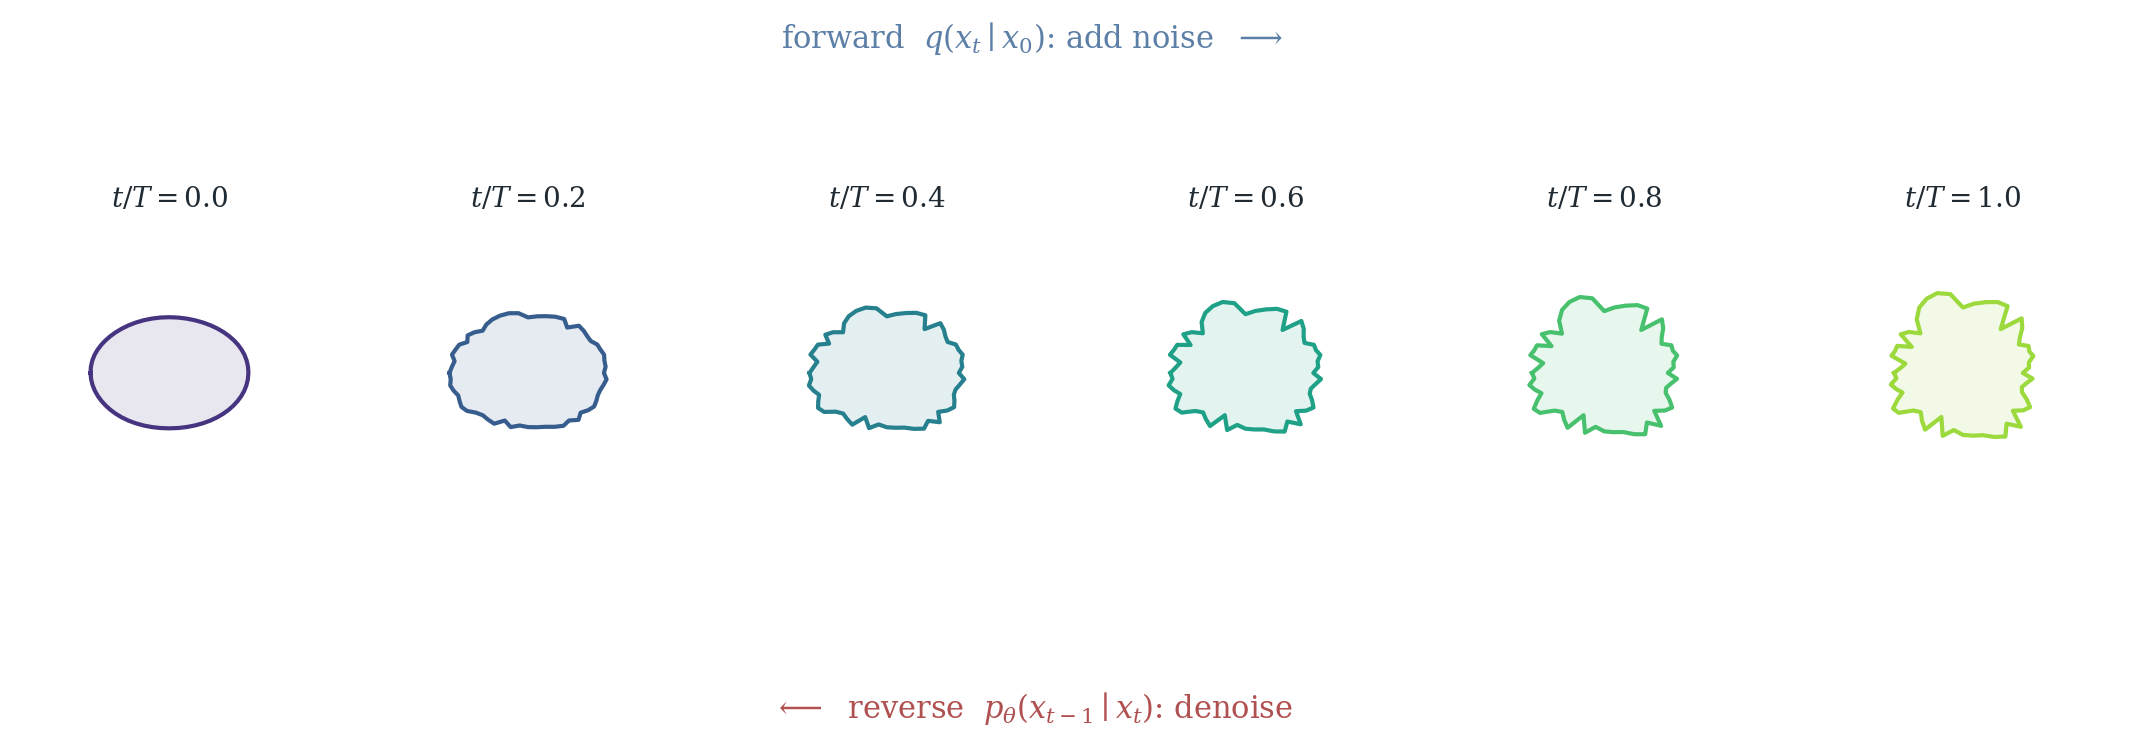
\includegraphics[width=0.95\linewidth]{report_diffusion_process.png}
  \caption{Forward and reverse diffusion on the radial field $r(\theta)$ of a real generated boundary.
  The forward process $q(x_t \mid x_0)$ progressively corrupts a clean shape (left) toward isotropic
  noise (right) along the cosine schedule; the learned reverse process denoises back, recovering
  surface detail in the final low-noise steps.}
  \label{fig:diffusion-process}
\end{figure}

\subsection{Graph-network score model}

The score network $\varepsilon_\theta$ stacks $N$ Battaglia-style graph-network blocks
\cite{battaglia2018relational}, each applying the canonical three-stage update ---
$\phi^e \to \phi^v \to \phi^u$ --- and aggregating messages along the bidirectional ring edges of
the boundary. The key design choice is how time and conditioning enter the network: the timestep is
mapped through a sinusoidal embedding, and both this embedding and the conditioning vector are
injected \emph{once} into the per-graph global attribute $u$, rather than being concatenated onto
every node. They then propagate to the nodes through the $\phi^u \to \phi^v$ message-passing
pathway, so a single per-graph signal conditions all nodes consistently and the per-node feature
stays a single radial channel. The model is implemented under a strict one-way package dependency
DAG (\texttt{building\_blocks/} $\to$ \texttt{model/}, with \texttt{data/} independent of both),
keeping the score architecture decoupled from data handling.

\begin{figure}[t]
  \centering
  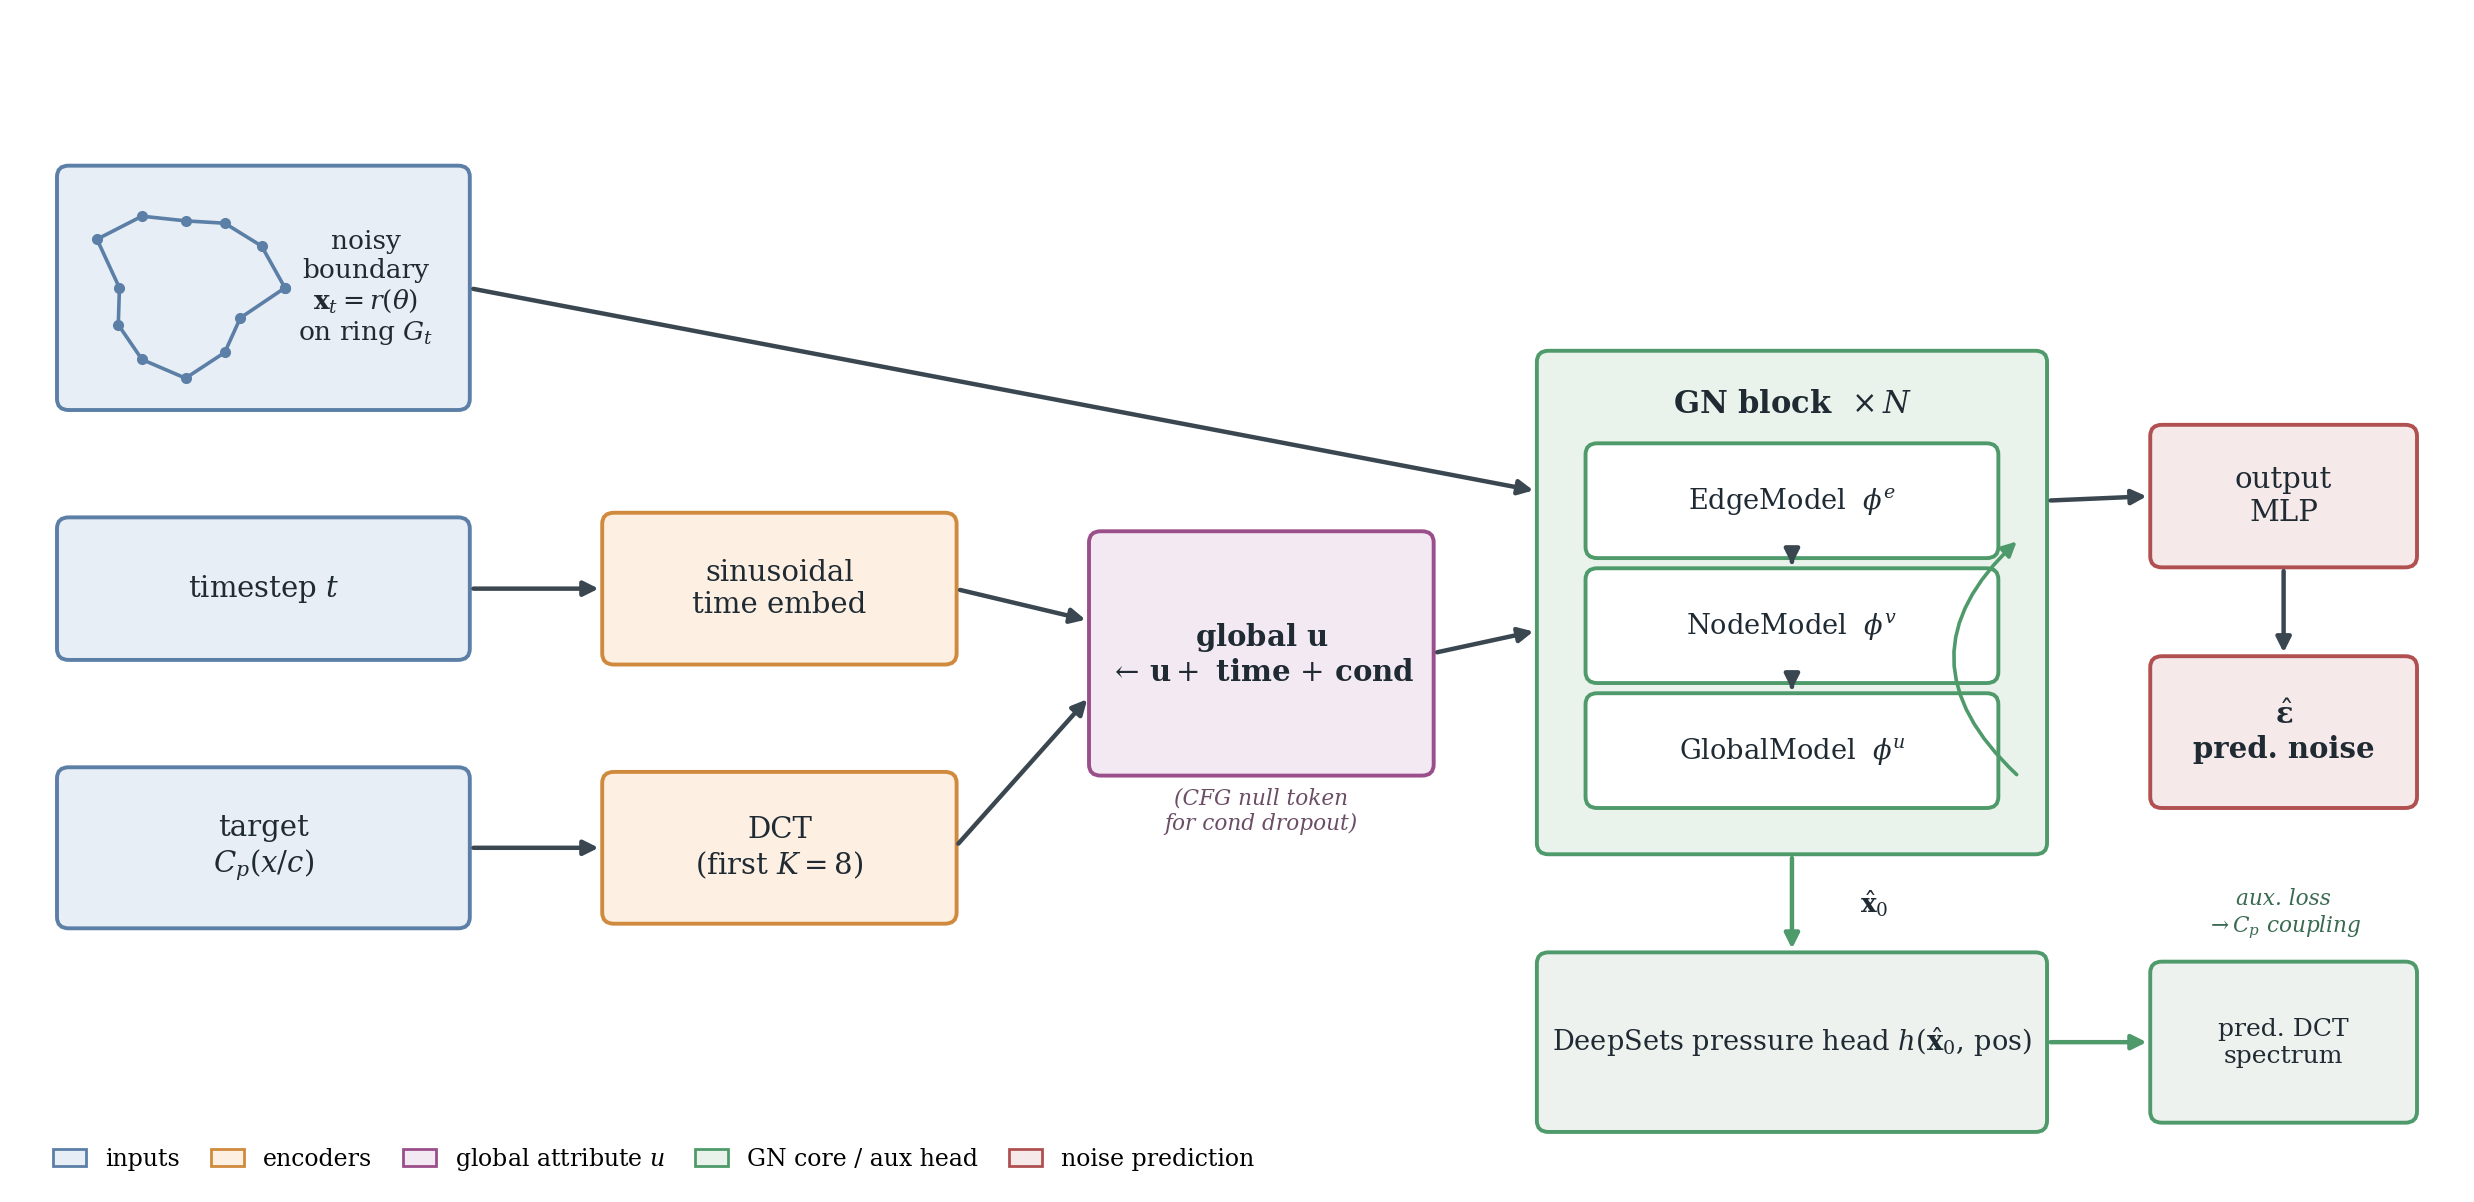
\includegraphics[width=0.8\linewidth]{report_architecture.png}
  \caption{Architecture of the score network $\varepsilon_\theta$. The diffusion timestep (via a
  sinusoidal embedding) and the DCT pressure-conditioning vector are summed once into the per-graph
  global attribute $u$, which feeds the $N\times$ stack of graph-network blocks
  ($\phi^e \to \phi^v \to \phi^u$) operating over the bidirectional ring edges; a
  jointly-trained auxiliary DeepSets pressure head reads the denoised shape to predict its pressure
  spectrum (detailed in Section~3.5).}
  \label{fig:architecture}
\end{figure}

\subsection{Pressure conditioning}

The target pressure curve is encoded compactly: we take the first $K=8$ type-II discrete cosine
transform (DCT) coefficients of the steady-mean $C_p(x/c)$. This yields a fixed-size conditioning
vector that is independent of the surface node count and captures the smooth, low-frequency
morphology of the pressure curve in a handful of numbers. Encoding alone, however, does not force
the model to respect physics. To tie geometry to pressure, a DeepSets pressure head
\cite{zaheer2017deepsets} $h(\hat{x}_0, \mathrm{pos}) \to \mathbb{R}^K$ is trained jointly with
the score network: from the denoised shape it must predict the DCT spectrum of the pressure that the
\emph{generated} shape would actually produce. Its prediction error supplies an auxiliary gradient
that couples the generated geometry to its implied pressure, forcing the model to learn the forward
shape$\to$pressure map rather than memorise training shape--pressure pairs. The DeepSets form is
chosen because it is permutation-invariant over the unordered set of surface nodes, matching the
symmetry of the boundary.

\begin{figure}[t]
  \centering
  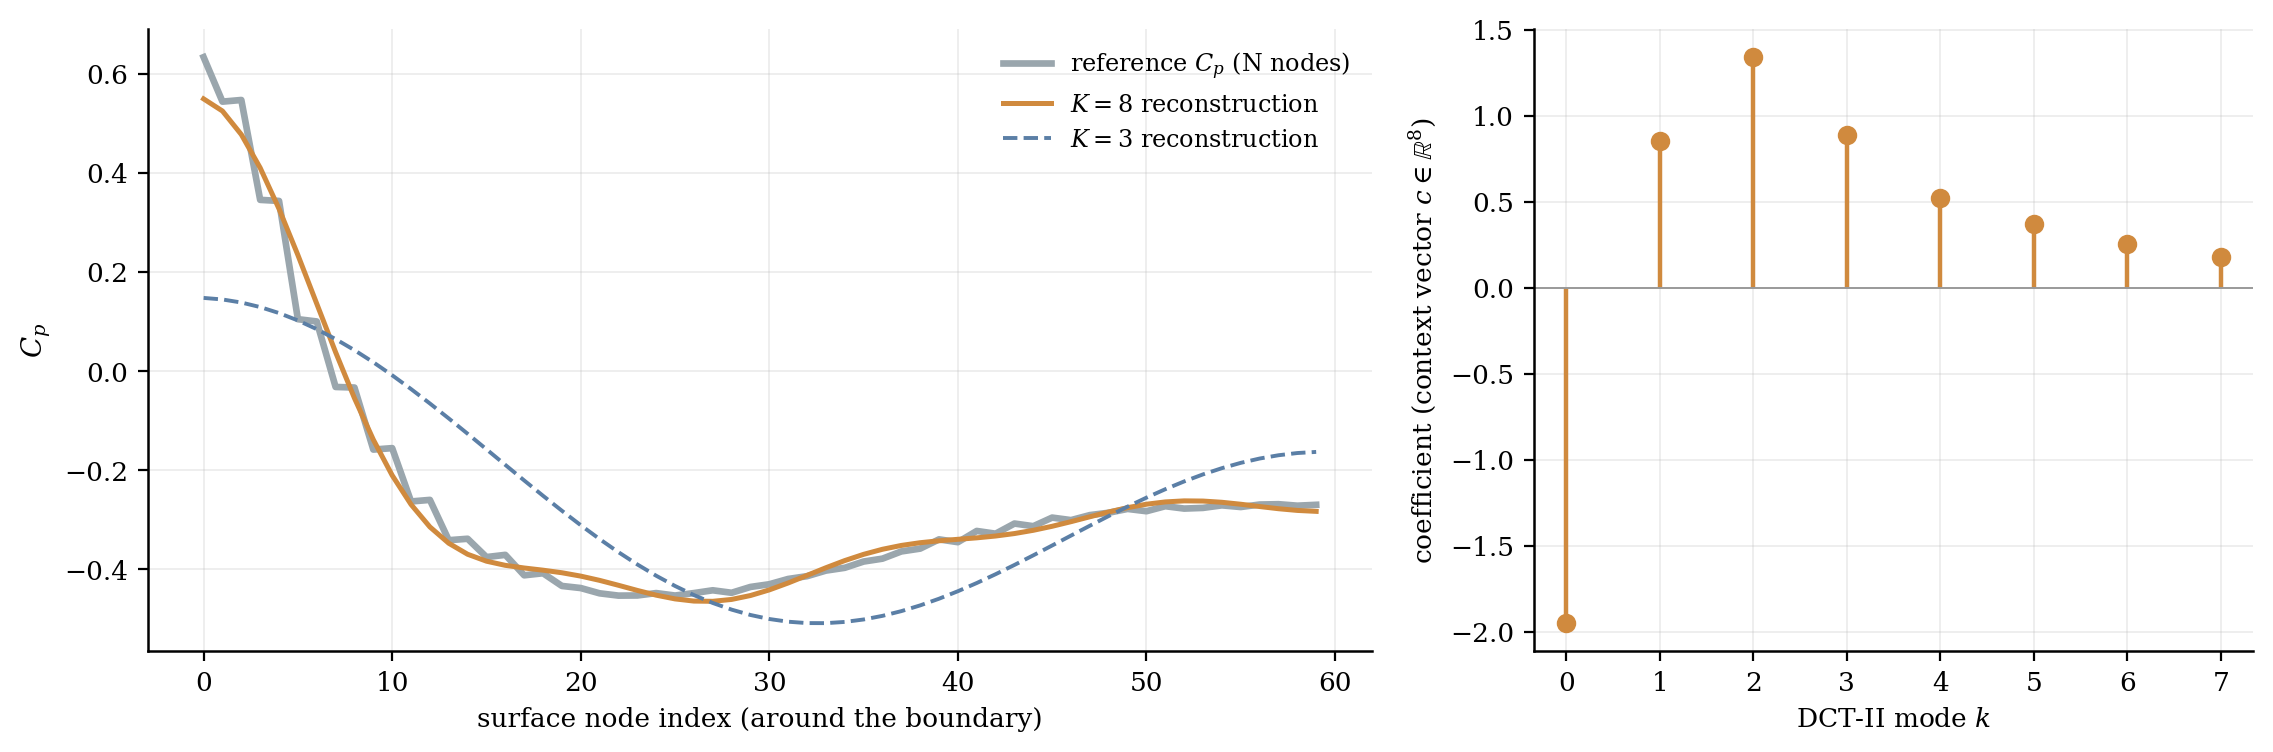
\includegraphics[width=0.85\linewidth]{report_dct_encoding.png}
  \caption{A real reference pressure sequence (grey) and its truncated DCT-II reconstruction. Eight
  modes ($K=8$, orange) recover the pressure morphology closely, while three modes (blue dashed) are
  visibly too coarse, motivating $K=8$ as a compact, node-count-independent conditioning vector.
  Right: the eight coefficients constituting the context vector $c$.}
  \label{fig:dct-encoding}
\end{figure}

\begin{figure}[t]
  \centering
  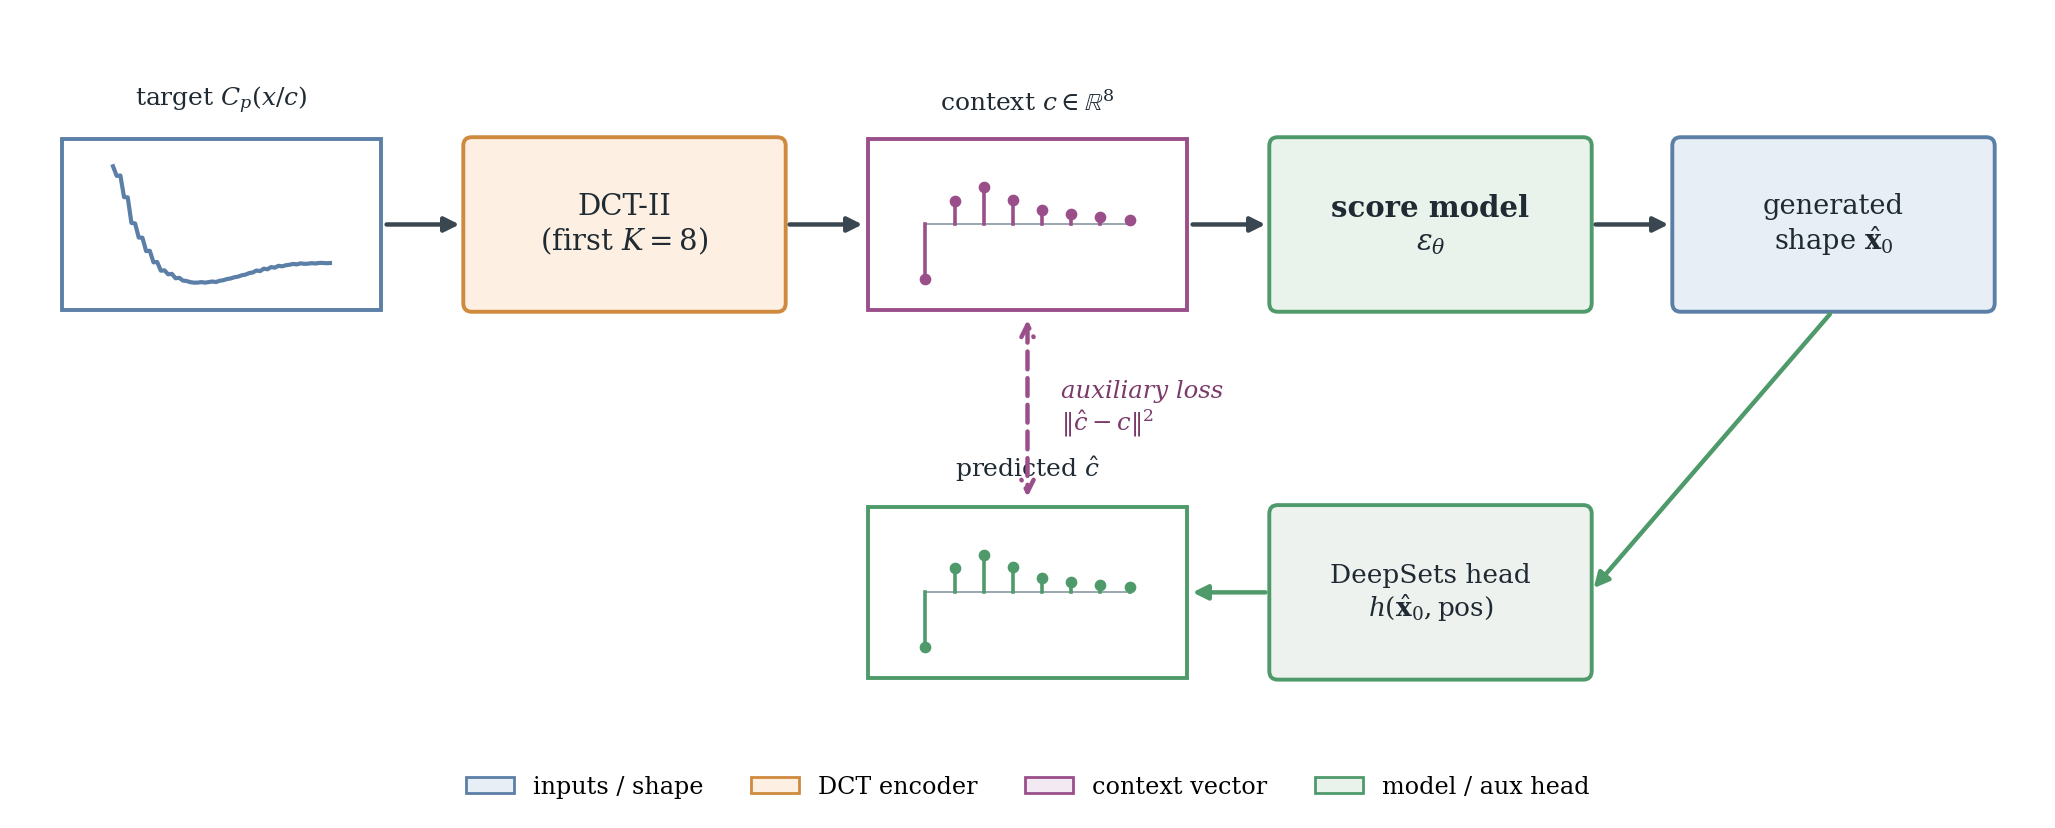
\includegraphics[width=0.95\linewidth]{report_conditioning_pipeline.png}
  \caption{The pressure-conditioning data flow. The target $C_p(x/c)$ is DCT-encoded into the
  fixed-size context $c$ that conditions the score model; the jointly-trained DeepSets head reads the
  generated shape and predicts its pressure spectrum $\hat{c}$, and the auxiliary loss
  $\lVert \hat{c} - c \rVert^2$ couples generated geometry back to pressure.}
  \label{fig:conditioning-pipeline}
\end{figure}

\subsection{Inference guidance}

At sampling time the conditioning signal is amplified with classifier-free guidance \cite{ho2022cfg}.
During training the condition is randomly dropped and replaced by a learnable null token, so the
same network learns both conditional and unconditional noise prediction. At inference the two
predictions are combined,

\begin{equation}
  \varepsilon = (1 + w)\cdot\varepsilon_\mathrm{cond} - w\cdot\varepsilon_\mathrm{uncond},
\end{equation}

with guidance weight $w$ (here $w=3.0$), pushing samples toward the target without a separate
classifier. The tested alternative is Diffusion Posterior Sampling \cite{chung2023dps}, which
instead adds a likelihood gradient from the jointly-trained pressure head to steer the reverse
process toward the measured target; its effect on out-of-distribution targets is reported in the
Results.

\subsection{Independent CFD validation solver}

Generated shapes are graded by an independent computational fluid dynamics solve rather than by the
model's own pressure head. The validation loop is a 2D incompressible lattice-Boltzmann solve
\cite{kruger2017lbm} built on OpenLB \cite{latt2021openlb}. The generated boundary polygon is
stamped into the lattice as a solid via a winding-number signed-distance indicator, giving a curved
Bouzidi no-slip body wall; the domain spans a velocity inlet, free-stream-velocity Dirichlet
conditions on the top and bottom walls, and a pressure outlet, with the channel height $H$ taken
from the dataset and the body centred at the half-height $H/2$. A graded sponge / absorbing layer
\cite{xu2013sponge} sits upstream of the outlet to suppress reflected acoustic waves that would
otherwise contaminate the measured field. The decisive property is independence: the solver measures
the time-averaged surface $C_p(x/c)$ from first principles and never sees the diffusion model or its
pressure head. Because the grading physics shares no component with the generator, a high
measured-versus-target correlation is a genuine physical confirmation of inverse design, not a
surrogate grading itself.

\begin{figure}[t]
  \centering
  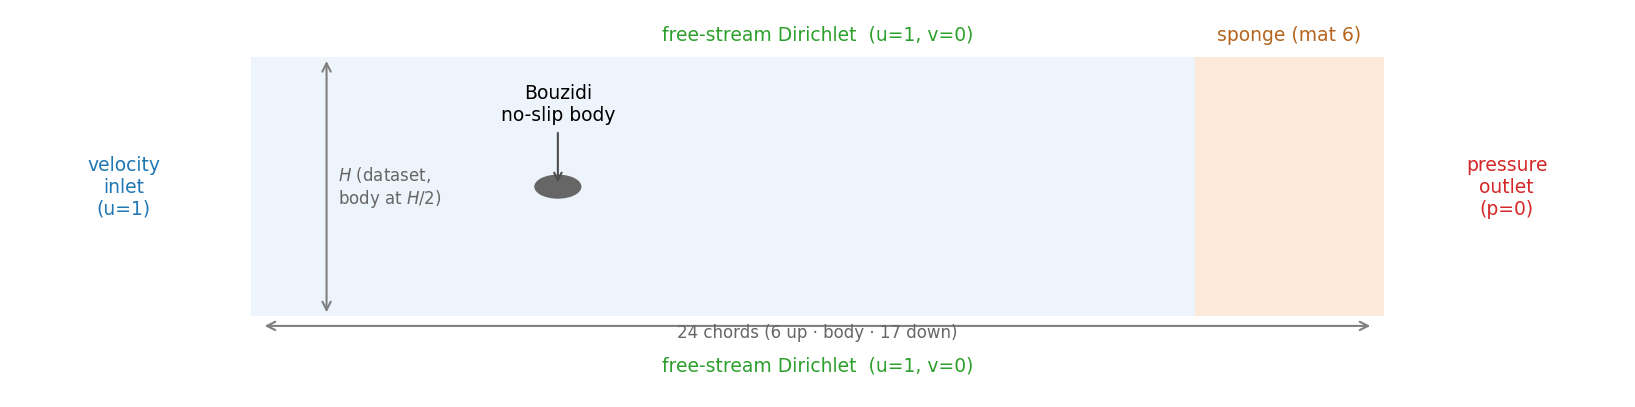
\includegraphics[width=0.8\linewidth]{EXP-043_domain_schematic.png}
  \caption{Schematic of the 2D lattice-Boltzmann validation domain: a velocity inlet, free-stream
  Dirichlet top and bottom walls, the stamped solid body with a curved Bouzidi no-slip wall centred
  at the dataset channel half-height $H/2$, and a pressure outlet preceded by a graded sponge layer.}
  \label{fig:domain-schematic}
\end{figure}

\paragraph{Key implementation details.} The solver is built on OpenLB 1.9.0 with a \texttt{D2Q9}
lattice and plain BGK collision (the target $Re$ 500--1000 is laminar, so no turbulence model). Five
elements fix the physics, and the code below shows how each is set up.

\paragraph{Reynolds number via viscosity.} The characteristic free-stream speed is held fixed at
$U = 1$ and the chord at $L = 1$; Reynolds number enters only through the physical viscosity
$\nu = U L / Re$, so $Re$ is decoupled from the inlet velocity. The unit converter is seeded from the
spatial resolution and the lattice relaxation time $\tau = 0.545$ (just above the BGK stability floor
of 0.5):

\begin{lstlisting}[style=cpp]
lattice.setUnitConverter<UnitConverterFromResolutionAndRelaxationTime<T,DESCRIPTOR>>(
    resolution,                          // voxels per chord  (RES ~ 0.2*Re for stability)
    latticeRelaxationTime,               // tau = 0.545   (> 0.5 BGK floor)
    charPhysLength,                      // L = chord = 1
    charPhysVelocity,                    // U = 1 m/s   (fixed)
    charPhysVelocity*charPhysLength/Re,  // nu = U*L/Re  <- Reynolds enters here
    physDensity);
\end{lstlisting}

Because the Mach number $\mathrm{Ma} = U_\mathrm{lattice}/c_s$ must stay $\lesssim 0.1$ for
incompressibility while the cell viscosity falls with $Re$, the grid resolution is scaled with Reynolds
number, $\mathrm{RES} \approx 0.2\,Re$, to keep the lattice viscosity in a stable band across the whole
regime.

\paragraph{Domain and channel height.} The domain spans $6 + 1 + 17 = 24$ chords streamwise (inlet 6
chords upstream of the body, outlet 17 downstream); the cross-stream extent is the dataset channel
height $H$ (5--6), and the body is centred at the half-height $H/2$, matching the dataset blockage ratio
rather than being free-chosen:

\begin{lstlisting}[style=cpp]
const T physDeltaX  = chord / resolution;
const T physLengthX = (upstreamChords + 1 + downstreamChords) * chord;  // 6 + 1 + 17 chords
const T physLengthY = H + physDeltaX;                    // channel height H (dataset 5-6)
const T shiftY      = (physLengthY / 2) - body.centroid[1];   // body centred at H/2
\end{lstlisting}

The channel height is a required input with no default --- an omitted \texttt{--CHANNEL\_HEIGHT} aborts
the run (a $-1.0$ sentinel $+$ a guard), so a wrong-domain run cannot pass silently.

\paragraph{Material map and boundary conditions.} The geometry is tagged with six material numbers ---
bulk fluid (1), free-stream top/bottom (2), velocity inlet (3), pressure outlet (4), the body (5), and
an absorbing sponge band (6) --- and each gets its dynamics or boundary condition:

\begin{lstlisting}[style=cpp]
dynamics::set<BGKdynamics>(lattice, geometry.getMaterialIndicator({1}));  // bulk
boundary::set<boundary::InterpolatedVelocity>(lattice, geometry, 3);      // inlet  (U, 0)
boundary::set<boundary::InterpolatedVelocity>(lattice, geometry, 2);      // free-stream top/bottom
boundary::set<boundary::InterpolatedPressure>(lattice, geometry, 4);      // outlet p = 0
setBouzidiBoundary(lattice, geometry, 5, *placedShape);                   // curved no-slip body
\end{lstlisting}

\paragraph{Body stamping.} The generated boundary polygon is turned into a solid by a hand-written
signed-distance indicator: the sign comes from a winding-number point-in-polygon test (robust for
non-convex shapes) and the magnitude from the nearest-edge distance, giving the true signed distance
(negative inside) that the curved Bouzidi wall reconstruction needs:

\begin{lstlisting}[style=cpp]
const T sign = (windingNumber % 2 == 1) ? -1 : +1;   // odd crossings => inside
return sign * nearestEdgeDistance;                   // negative inside, positive outside
\end{lstlisting}

\paragraph{Surface $C_p$ from a time-averaged field.} Because the flow sheds vortices, a single-step
pressure readout is meaningless; the solver discards the start-up transient and accumulates a
time-averaged pressure field over a window spanning many shedding periods. The surface $C_p(x/c)$ is
then probed half a cell outside each boundary node along its outward normal, and referenced to the
undisturbed free-stream static pressure (sampled $0.4\,H$ above the body) rather than the outlet gauge,
so the stagnation point reads $C_p \approx 1$:

\begin{lstlisting}[style=cpp]
const T qInf = 0.5 * rho * U * U;                     // dynamic pressure
const Vector<T,2> probe{ node[0] + 0.5*dx*nrm[0],     // 0.5*dx outside the surface,
                         node[1] + 0.5*dx*nrm[1] };   // along the outward normal
Cp = (p_timeAveraged(probe) - p_inf) / qInf;          // p_inf from a free-stream probe
\end{lstlisting}

A graded sponge / absorbing layer \cite{xu2013sponge} (material 6) just upstream of the outlet, together
with rest-initialisation and a smooth inlet velocity ramp, suppresses reflected pressure waves so the
averaging window sees a clean periodic signal.

\subsection{Dataset}

Training data is the pOnEllipse dataset \cite{lino2022msgnn}: 2D incompressible flow around an
elliptical cylinder of major-axis length 1 (semi-major 0.5), with variable minor axis $b$ and
channel height $H$, at Reynolds numbers 500--1000 --- the laminar vortex-shedding regime. It
comprises 5701 training simulations, each storing per-surface-node coordinates together with 101
unsteady pressure timesteps, which we collapse to a single steady-mean $C_p$. The per-node HDF5
layout is \texttt{[x, y, Re, H, p0..p100]}. Note that the fourth column $H$ is the channel height
($\approx 5$--6), not angle of attack --- a distinction that matters because mistaking it for AoA
would corrupt the conditioning. The narrow, well-characterised regime makes this dataset a
controlled testbed for inverse design before scaling to higher-Reynolds or 3D flows.

\begin{figure}[t]
  \centering
  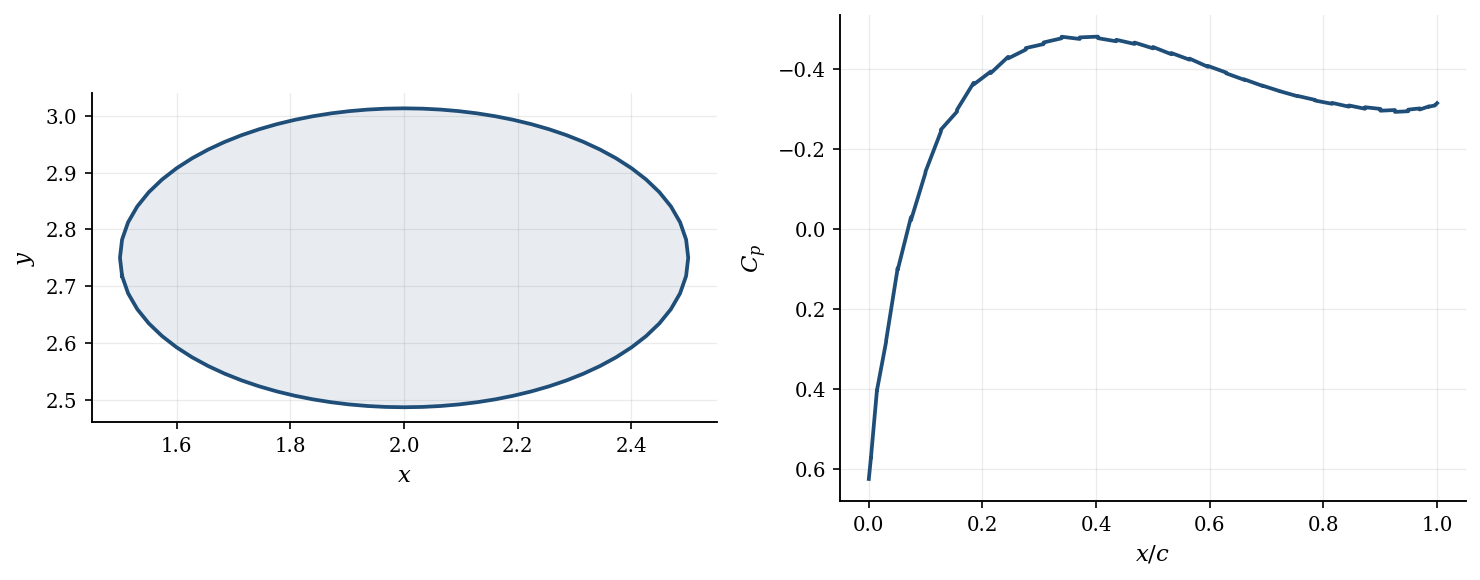
\includegraphics[width=0.8\linewidth]{report_dataset_example.png}
  \caption{An example pOnEllipse training sample: a closed elliptical boundary (left) and its
  corresponding steady-mean surface pressure curve $C_p(x/c)$ (right), the quantity the model is
  conditioned on.}
  \label{fig:dataset-example}
\end{figure}

The dataset spans a two-parameter design space --- Reynolds number $Re$ and semi-minor axis $b$ ---
sampled densely across the laminar regime, with the geometry varying smoothly with $b$.

\begin{figure}[t]
  \centering
  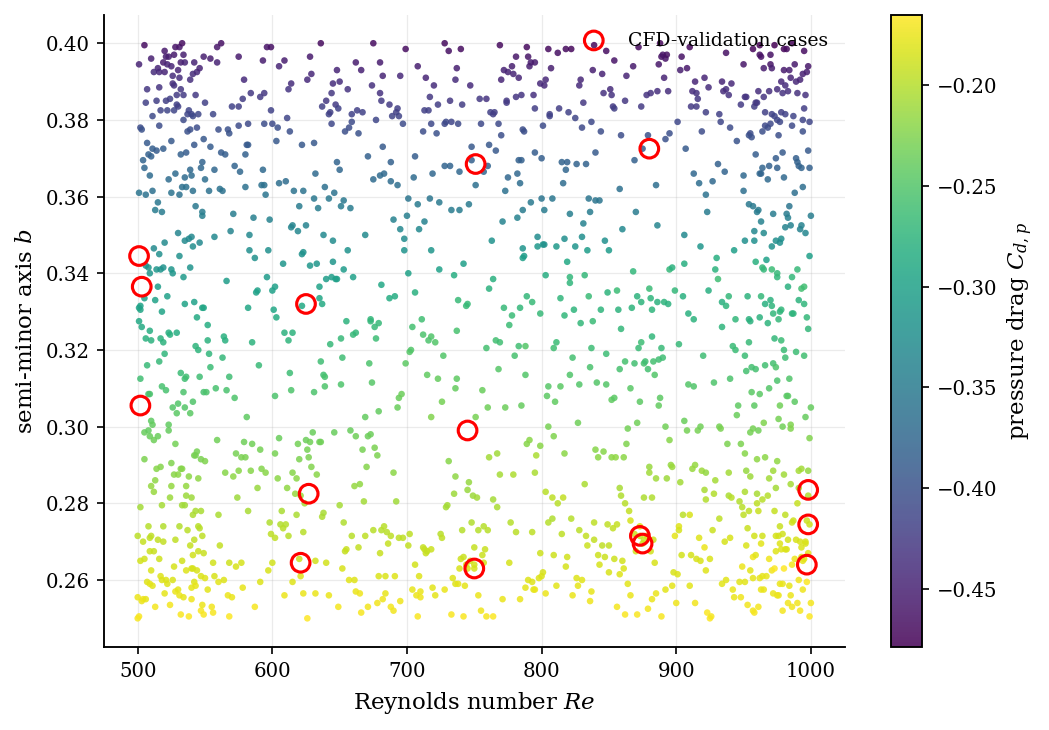
\includegraphics[width=0.7\linewidth]{report_design_space.png}
  \caption{Design-space coverage of the training set: each point is one simulation in the $(Re, b)$
  plane, coloured by its pressure drag. Sampling is dense and near-uniform across the regime; the
  circled points mark the cases later put through the CFD validation loop.}
  \label{fig:design-space}
\end{figure}

The conditioning targets the model sees --- the steady-mean $C_p(x/c)$ curves --- form a structured
family whose morphology is dominated by the minor axis $b$ rather than by $Re$: thinner bodies
(small $b$) develop a deeper suction trough, while $Re$ mainly modulates the wake recovery.

\begin{figure}[t]
  \centering
  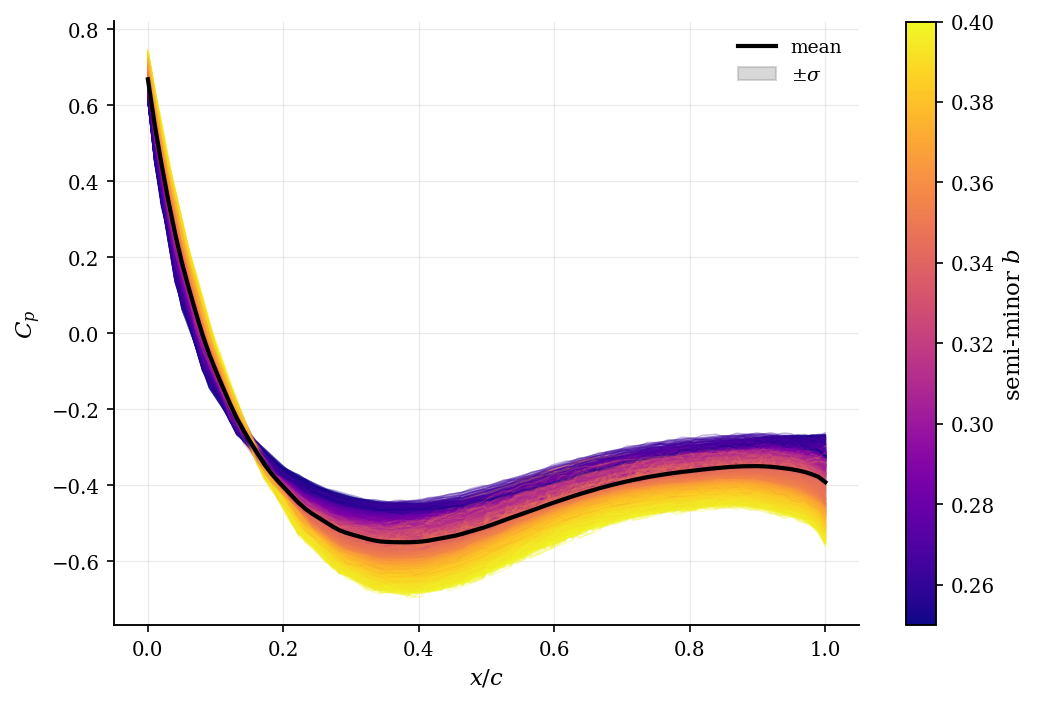
\includegraphics[width=0.7\linewidth]{report_cp_envelope.png}
  \caption{Surface-pressure target distribution across the whole training set, every curve coloured
  by its minor axis $b$ (mean $\pm\,\sigma$ in black). The systematic ordering with $b$ shows that
  $b$ is the principal driver of pressure morphology --- the low-frequency structure the DCT
  conditioning is designed to capture.}
  \label{fig:cp-envelope}
\end{figure}

\subsection{Evaluation metrics}

The headline verdict for inverse design is the \textbf{Pearson correlation} between the
solver-measured $C_p(x/c)$ and the conditioning target: it scores whether the generated shape
reproduces the \emph{shape} of the target pressure curve (its morphology), independently of
amplitude. We report it as the primary metric because the model captures $C_p$ shape, not absolute
magnitude. Alongside it we report the affine slope $a$ and offset $b$ from a linear fit of measured
against target $C_p$, which quantify amplitude calibration; the drag coefficient $C_d$; and the
second-difference roughness of $r(\theta)$, a surface-quality measure where lower is smoother. We
state explicitly that correlation, not absolute amplitude, is the inverse-design verdict --- the
affine slope is reported as a known calibration limitation rather than a pass/fail criterion.

\paragraph{Definition and computation.}
Both metrics are computed on a common abscissa: the solver-measured curve is first interpolated onto
the reference $x/c$ grid so the comparison is point-for-point. Writing the reference samples as $x_i$
and the measured samples as $y_i$ (with means $\bar{x}, \bar{y}$), the Pearson correlation is
\begin{equation}
  \rho \;=\; \frac{\sum_i (x_i - \bar{x})(y_i - \bar{y})}
                  {\sqrt{\sum_i (x_i - \bar{x})^2}\,\sqrt{\sum_i (y_i - \bar{y})^2}},
  \qquad \rho \in [-1, 1],
  \label{eq:pearson}
\end{equation}
the mean-centred, variance-normalised inner product of the two curves. The affine slope and offset are
the least-squares solution of $y \approx a\,x + b$; $a$ is the magnitude scaling and $b$ the constant
offset, and the affine-residual RMS --- the error remaining once the best $a, b$ are removed ---
isolates the part of the mismatch that scaling and offset cannot explain.

\paragraph{Invariance of $\rho$ to the affine fit.}
Pearson correlation is invariant under a positive affine transformation of either variable, which is
exactly why it and the affine fit measure complementary things. Replacing $y$ with the fitted
$a\,y + b$, the covariance scales linearly while the constant drops out,
$\operatorname{cov}(x, a\,y + b) = a\,\operatorname{cov}(x, y)$, and the standard deviation scales by
$|a|$, $\sigma_{a y + b} = |a|\,\sigma_y$, so $\rho(x, a\,y + b) = \operatorname{sign}(a)\,\rho(x, y)$:
for $a > 0$ the slope and offset cancel exactly. Equivalently, the mean-centring in the numerator of
Eq.~\eqref{eq:pearson} annihilates the offset $b$ and the $\sigma$-normalisation in the denominator
annihilates the scale $a$. Correlation is therefore blind, by construction, to overall magnitude and
offset, grading only the \emph{shape} of the pressure distribution, while the affine slope $a$ captures
exactly what $\rho$ discards. The two are reported together and fail independently: a result such as
$\rho \approx 0.999$ with $a \approx 1.87$ reads as ``near-perfect shape agreement at ${\approx}1.87\times$
the reference amplitude.'' Reporting $\rho$ alone would conceal that amplitude offset --- the
\emph{magnitude creep} characterised in Section~\ref{sec:ood} (where $a$ drifts above its validated
${\approx}1.74$ baseline while $\rho$ stays high).

\section{Results}

\begin{quote}
\textbf{Note on preliminary material.} The two studies below are \emph{preliminary} --- on a canonical
benchmark and an exploratory surface metric --- and fixed design choices carried into the rigorous
aerodynamic validation that follows. They are summarised compactly here; how each would be put on a
rigorous footing is set out in Section~\ref{sec:toward-rigour}.
\end{quote}

\subsection{Preliminary: representation and connectivity}

A canonical circle-series study fixed two design choices reused unchanged downstream: a single-scalar
radial node feature $[r]$ (rather than coupled Cartesian channels), and the ring-graph connectivity.
The connectivity was settled by an ablation sweeping the neighbours-per-side $k \in \{1, 2, 4, 6\}$ with
everything else fixed (4-layer GN, $T = 200$, 50 epochs), graded by the Kolmogorov--Smirnov (KS)
distance between the generated and reference radius distributions (lower is better).

% source: k-neighbour ablation, EXP-002, outputs/EXP-002{a,b,c,d}/evaluation_report.json
\begin{table}[t]
  \centering
  \begin{tabular}{lcc}
    \toprule
    Ring connectivity $k$ & KS statistic ($\downarrow$) & val loss \\
    \midrule
    1 (nearest-neighbour only) & 0.215          & 0.0642          \\
    2                          & 0.193          & 0.0403          \\
    4                          & 0.160          & 0.0414          \\
    6                          & \textbf{0.094} & \textbf{0.0378} \\
    \bottomrule
  \end{tabular}
  \caption{Ring-connectivity ablation on the circle benchmark (EXP-002): KS distance to the reference
  radius distribution and validation loss against neighbours per side $k$.}
  \label{tab:connectivity}
\end{table}

The KS distance falls monotonically with connectivity --- a 56\% reduction from $k = 1$ to $k = 6$,
corroborated by the validation loss --- so $k = 6$ was adopted for all downstream work. This is a
single-seed study on the circle benchmark, not an aerodynamic-domain result
(Section~\ref{sec:toward-rigour}).

\subsection{Preliminary: surface quality}
\label{sec:surface-quality}

Generated boundaries carry a small high-frequency wobble. An exploratory study swept six
training/sampling configurations against a mean second-difference roughness of $r(\theta)$ (lower is
smoother) on four fixed targets, to locate where surface quality is controlled.

% provisional
\begin{table}[t]
  \centering
  \begin{tabular}{lcccc}
    \toprule
    Configuration & Diffusion steps $T$ & Overall roughness & $\Delta$ vs baseline & Best val loss \\
    \midrule
    baseline                                        & 200  & 0.03379            & ---       & 0.00306   \\
    longer training                                 & 200  & 0.02125            & $-$37\%   & 0.000104  \\
    longer training $+$ $T=1000$ steps              & 1000 & \textbf{0.01523}   & $-$55\%   & 0.000090  \\
    $+$ Min-SNR-$\gamma$ loss \cite{hang2023minsnr} & 200  & 0.02700            & $-$20\%   & \textbf{0.000028} \\
    $+$ EMA \cite{song2020improved}                 & 200  & 0.03747            & $+$11\%   & 0.000124  \\
    $+$ EMA $+$ v-prediction \cite{salimans2022progressive} & 200 & 0.02451     & $-$27\%   & 0.000189  \\
    \bottomrule
  \end{tabular}
  \caption{Surface-quality sweep: roughness and validation loss for six training/sampling
  configurations. Lower roughness is smoother; bold marks the winner in each column.}
  \label{tab:surface-quality}
\end{table}

The single takeaway is that boundary smoothness is a \emph{sampling-time} property: the $T = 1000$
configuration roughly halves roughness ($-55\%$) while its validation loss is essentially unchanged from
longer-training-alone, and the lowest-loss configuration (Min-SNR-$\gamma$) is \emph{not} the smoothest.
Minimising the training MSE harder does not smooth boundaries --- more reverse-diffusion steps do. This
used a non-standard roughness proxy on four targets and is treated as exploratory; a rigorous
surface-quality protocol is outlined in Section~\ref{sec:toward-rigour}. Critically, the downstream
validation shows this wobble is cosmetic: it does not corrupt the measured physics
(Section~\ref{sec:in-dist}).

\subsection{CFD solver validation gate}
\label{sec:solver-gate}

Before trusting the loop on generated shapes, we gate it on \emph{known} dataset ellipses run with the
corrected domain --- the channel height $H$ taken from the dataset (5--6) with the body centred at the
half-height $H/2$, rather than the earlier free-chosen height.\footnote{An earlier preliminary gate
used a free-chosen channel height that did not match the dataset's domain; those runs are superseded by
the corrected-domain validation reported here.} The independent solver reproduces the
dataset's own $C_p$ at correlation up to $\approx 1.0$, establishing that the grading physics is sound
before any generated geometry is judged by it. The validation calculation interpolates the (monotonic)
dataset reference $C_p$ onto the solver's surface nodes --- the solver $C_p$ traces the full closed
boundary and is non-monotonic in $x/c$ --- and reports the Pearson correlation and the affine fit
$\mathrm{measured} \approx a\cdot\mathrm{ref} + b$.

\begin{table}[t]
  \centering
  \begin{tabular}{lcccccc}
    \toprule
    Sim & Re & $H$ & $C_p$ correlation & affine slope $a$ & offset $b$ \\
    \midrule
    sim\_59   & 503 & 5.5 & 0.971          & 1.76 & 0.06 \\
    sim\_2824 & 750 & 5.5 & 0.944          & 1.73 & 0.07 \\
    sim\_5645 & 998 & 5.5 & \textbf{0.999} & 1.87 & 0.02 \\
    \bottomrule
  \end{tabular}
  \caption{CFD solver validation gate on three known dataset ellipses spanning the Reynolds-number
  range at $H = 5.5$, with the corrected channel height: $C_p$ correlation, affine slope, and offset.}
  \label{tab:solver-gate}
\end{table}

The solver reproduces the dataset curve up to a single multiplicative normalisation $a \approx 1.7$--1.9,
strikingly close to the dataset's documented ``u / 1.8'' velocity scaling --- a credible analytic
explanation rather than a solver artefact --- with a near-zero offset $b$. Correlation dips slightly at
the mid-Reynolds case through genuine under-resolution of the stronger vortex shedding, not a
correctness failure.

\begin{figure}[t]
  \centering
  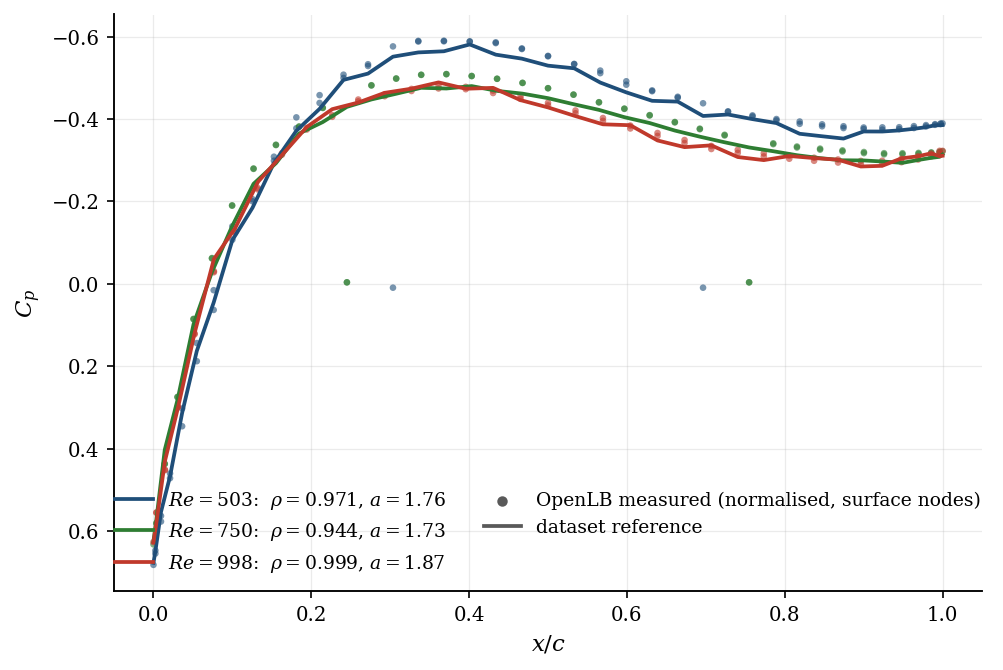
\includegraphics[width=0.8\linewidth]{EXP-043_cp_validation.png}
  \caption{Solver-measured surface pressure $C_p(x/c)$ (points, one per boundary node) against the
  dataset's own $C_p$ (solid lines) for three known ellipses spanning the Reynolds-number range at
  $H = 5.5$, with the corrected channel height. The measured nodes are mapped back into reference units
  by the per-case affine fit ($(\mathrm{measured} - b)/a$) so the shape agreement is shown directly; the
  amplitude $a \approx 1.7$--1.9 that is divided out --- the dataset's velocity normalisation --- is
  reported per curve in the legend.}
  \label{fig:cp-comparison}
\end{figure}

The measured $C_p$ is a time-average over a window spanning many shedding periods, and it is
well-converged: the per-node temporal RMS stays small ($\leq 0.12$) and the integrated drag is steady
($C_d = 0.86 \pm 0.06$), so the surface pressure the loop grades is a stable quantity rather than an
instantaneous snapshot.

\begin{figure}[t]
  \centering
  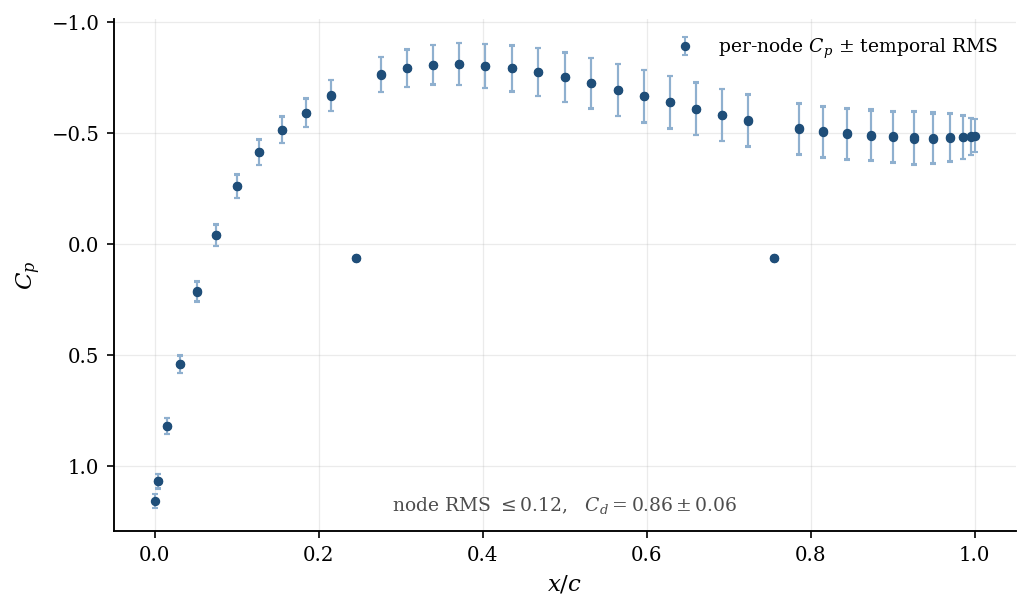
\includegraphics[width=0.8\linewidth]{EXP-043_cp_stability.png}
  \caption{Stabilisation of the surface $C_p$ for the mid-Reynolds case (Re = 750, $H = 5.5$): each
  marker is one boundary node's time-averaged $C_p$, with error bars showing the temporal RMS
  fluctuation over the averaging window. The small bands (node RMS $\leq 0.12$) and steady drag
  ($C_d = 0.86 \pm 0.06$) confirm the measured pressure is well-converged.}
  \label{fig:cp-stability}
\end{figure}

The three-ellipse spot-check is corroborated by a systematic gate over the whole design space. We
laid a 15-case grid across the dataset's $(Re, H)$ plane, snapping each grid node to its nearest real
simulation, and ran every case through the solver with per-case Reynolds-scaled resolution
($\mathrm{RES} \approx 0.2\,Re$); all 15 runs were numerically stable (no NaN, $\mathrm{avgRho}
\approx 1.0$, max CFL $\approx 0.1$).

\begin{table}[t]
  \centering
  \begin{tabular}{lcc}
    \toprule
    Quantity & Range across the 15-case grid & Mean \\
    \midrule
    $C_p$ correlation $\rho$ & 0.89 -- 1.00 & \textbf{0.96} \\
    affine slope $a$         & 1.51 -- 1.87 & \textbf{1.74} \\
    \bottomrule
  \end{tabular}
  \caption{Systematic 15-case solver-validation grid over the $(Re, H)$ design space: $C_p$
  correlation and affine slope range and mean.}
  \label{tab:eval-grid}
\end{table}

The mean slope $a \approx 1.74$ reproduces the three-ellipse normalisation ($a \approx 1.7$--1.9)
across the full $(Re, H)$ grid, confirming the single multiplicative factor is a stable property of the
solver --- the dataset's velocity normalisation --- and not an artefact of the three hand-picked cases.
With the gate holding at $\rho \approx 0.96$ everywhere in-distribution, \textbf{the solver is trusted
as physical ground truth for grading generated shapes.}

\begin{figure}[t]
  \centering
  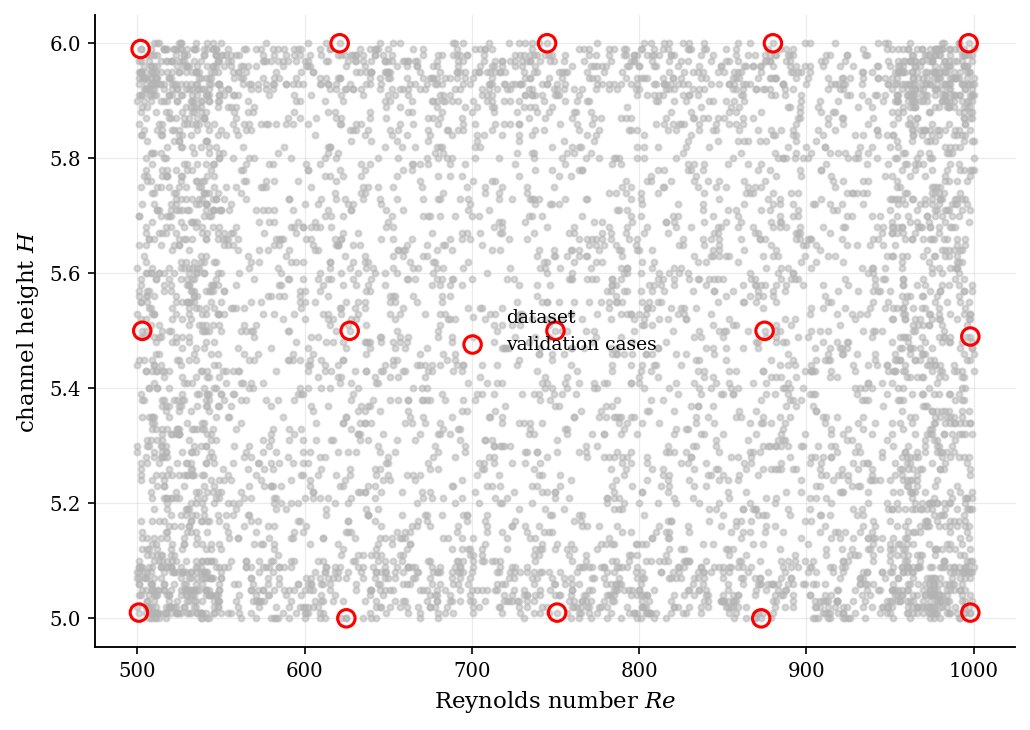
\includegraphics[width=0.8\linewidth]{EXP-043_eval_grid_coverage.png}
  \caption{The 15-case solver-validation grid laid over the training design space: each gate case
  (markers) is snapped to its nearest real simulation within the dataset $(Re, H)$ cloud, so the gate
  samples the whole regime rather than a few hand-picked points.}
  \label{fig:eval-grid-coverage}
\end{figure}

\subsection{In-distribution inverse design}
\label{sec:in-dist}

Generated shapes hit their target $C_p$ at correlation $\approx 0.95$ in-distribution, verified by
the independent solver rather than the model's own pressure head --- the first independent
confirmation of the inverse-design claim. Each shape is sampled for a dataset-drawn target $C_p$, run
through the validated loop, and its measured $C_p$ correlated against that target.

\begin{table}[t]
  \centering
  \begin{tabular}{lccc}
    \toprule
    Target & Re & $C_p$ corr (raw) & $C_p$ corr (smoothed) \\
    \midrule
    \#4849 & 960 & \textbf{0.964} & 0.952 \\
    \#4066 & 884 & \textbf{0.966} & 0.963 \\
    \bottomrule
  \end{tabular}
  \caption{In-distribution inverse-design validation: solver-measured $C_p$ correlation against the
  conditioning target for two generated shapes.}
  \label{tab:inverse-design}
\end{table}

Morphology is reproduced closely ($\rho \approx 0.95$--0.97), and the surface wobble of
Section~\ref{sec:surface-quality} proves cosmetic: raw versus Fourier-smoothed shapes differ by only
$\Delta\rho \sim 0.01$ in $C_p$ and $\sim 5\%$ in $C_d$, so it does not corrupt the measured physics.
Correlation --- not absolute amplitude --- is the verdict here: the model captures $C_p$ \emph{shape},
while its amplitude calibration (the affine slope) is a known limitation quantified on a controlled axis
in Section~\ref{sec:ood}.

\begin{figure}[t]
  \centering
  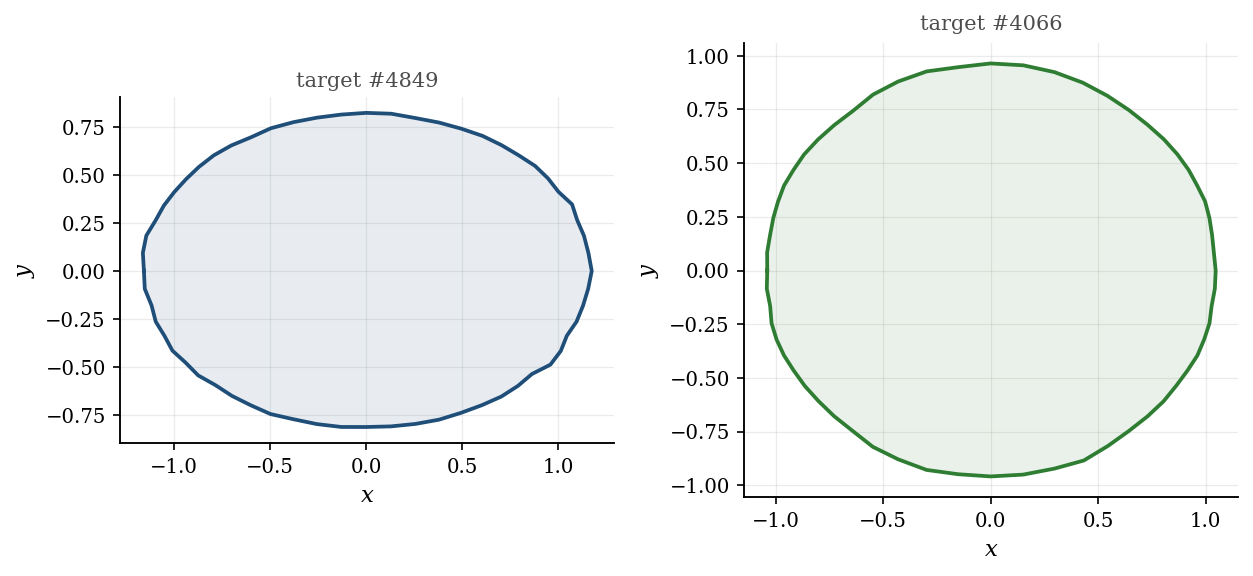
\includegraphics[width=0.8\linewidth]{report_generated_shapes.png}
  \caption{Boundaries generated by the conditional model for the in-distribution validation targets,
  before CFD grading.}
  \label{fig:generated-shapes}
\end{figure}

\begin{figure}[t]
  \centering
  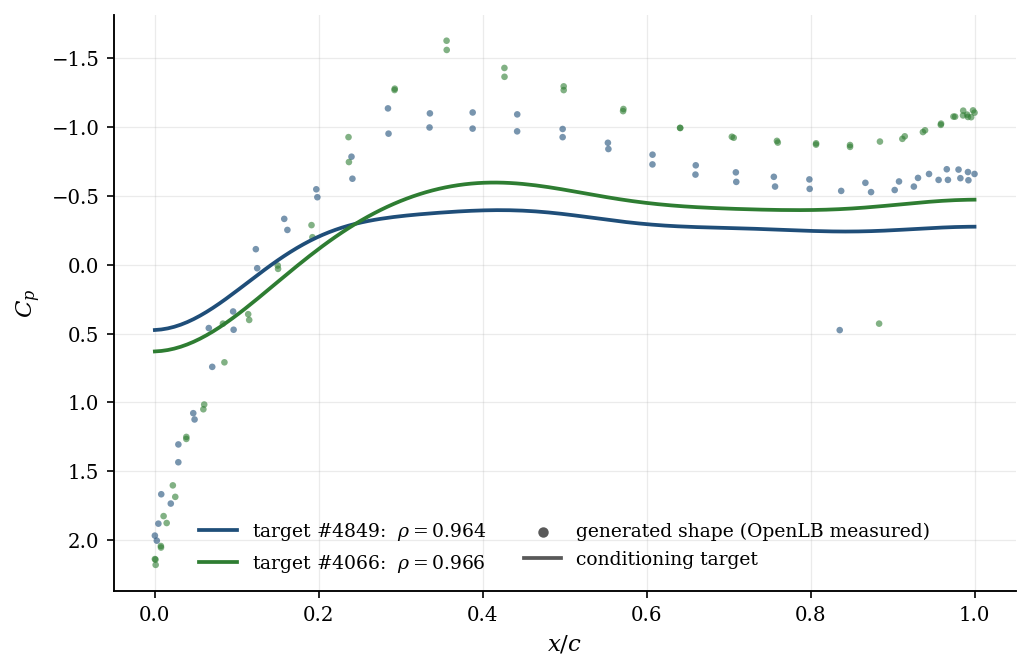
\includegraphics[width=0.8\linewidth]{EXP-041_cp_inverse_design.png}
  \caption{Solver-measured $C_p(x/c)$ of each generated in-distribution shape overlaid on its
  conditioning target: the morphology tracks closely.}
  \label{fig:cp-inverse-design}
\end{figure}

\subsection{Out-of-distribution behaviour and magnitude creep}
\label{sec:ood}

Out of distribution, inverse-design fidelity degrades --- the failure mode the independent loop was
built to surface. An initial five-target ad-hoc probe first exposed this; we report the
\textbf{controlled successor} that supersedes it. The OOD axis is made principled by perturbing the
dataset-mean $C_p$ along the dataset's own principal pressure modes,
\[
  C_p^{\mathrm{target}}(x) = \overline{C_p}(x) + s \cdot \alpha \cdot \sigma_m \cdot \mathrm{PC}_m(x),
\]
for modes $m \in \{\mathrm{PC1}, \mathrm{PC2}\}$, amplitudes $\alpha \in \{1, 2, 3, 4\}$ $\sigma$-units,
and both signs $s$ (16 targets). Each is generated with plain classifier-free guidance at fixed
$Re/H = 754/5.5$ --- so target morphology is the only variable --- and graded through the validated
solver (all 16 runs stable).

\begin{table}[t]
  \centering
  \begin{tabular}{cccc}
    \toprule
    amplitude $\alpha$ ($\sigma$) & OOD distance & $C_p$ corr $\rho$ & affine slope $a$ \\
    \midrule
    1 & 1.80 & 0.901          & 2.08 \\
    2 & 2.02 & 0.922          & 2.06 \\
    3 & 2.33 & 0.858          & 1.79 \\
    4 & 2.74 & \textbf{0.857} & 1.76 \\
    \bottomrule
  \end{tabular}
  \caption{The genuinely-OOD $+\mathrm{PC1}$ ladder: $C_p$ correlation and affine slope against
  out-of-distribution distance as the target amplitude is pushed from 1 to 4$\sigma$.}
  \label{tab:ood-ladder}
\end{table}

Along the genuinely-OOD $+\mathrm{PC1}$ direction, correlation falls monotonically from $\sim 0.92$ to
$\sim 0.86$ as the target moves out. One parameterisation caveat --- itself a finding --- is that
\textbf{only $+\mathrm{PC1}$ is genuinely reachable as OOD}: the other principal directions stay near
the training manifold (OOD distance $\approx 1.0$--1.6) regardless of amplitude, because the raw-curve
PCA $\sigma$-units are not isometric to the DCT-conditioning space the model sees. A future ladder
should sweep amplitude in conditioning space directly (Section~\ref{sec:toward-rigour}).

\begin{figure}[t]
  \centering
  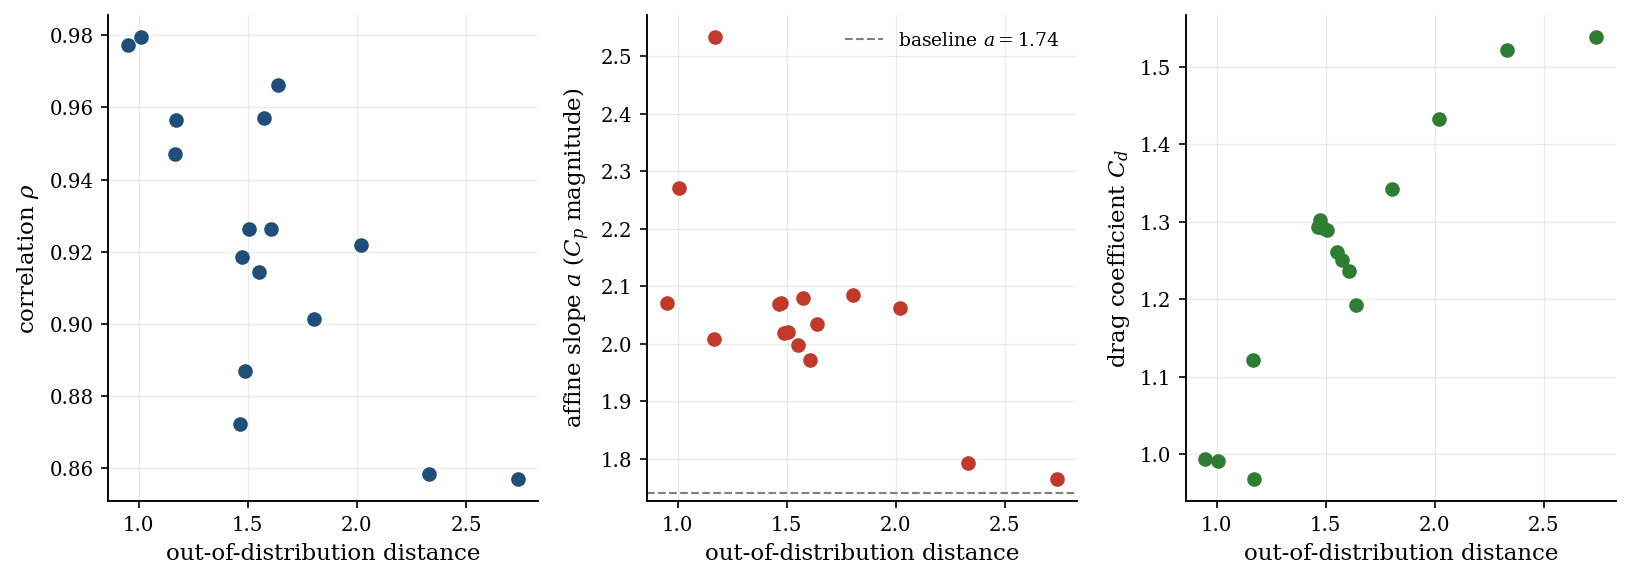
\includegraphics[width=0.95\linewidth]{EXP-043_ood_results_summary.png}
  \caption{Inverse-design fidelity against out-of-distribution distance across the 16-target ladder:
  correlation $\rho$ (left) softens, the affine slope $a$ (centre) sits above the validated 1.74
  baseline, and drag $C_d$ (right) rises with OOD distance.}
  \label{fig:ood-results-summary}
\end{figure}

\begin{figure}[t]
  \centering
  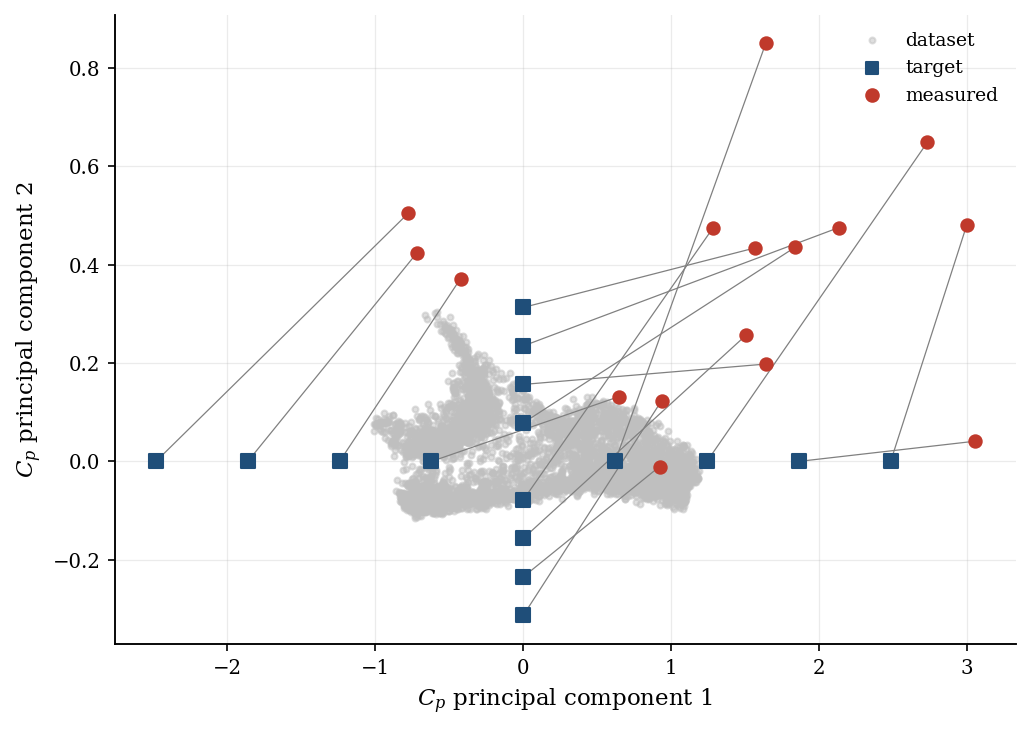
\includegraphics[width=0.8\linewidth]{EXP-043_ood_cp_manifold.png}
  \caption{The OOD ladder in the dataset's principal-component $C_p$ plane: training curves form the
  backdrop cloud; the $+\mathrm{PC1}$ targets march progressively outside it (making
  ``out-of-distribution'' concrete), while the other directions stay near the training manifold.}
  \label{fig:ood-cp-manifold}
\end{figure}

\paragraph{The amplitude bias is model-side.} Across all 16 OOD targets the affine slope spans
$a \approx 1.8$--2.5, above the solver's validated in-distribution baseline of 1.74
(Section~\ref{sec:solver-gate}). The point is sharpest when real dataset shapes and generated shapes are
graded by the \emph{same} solver: dataset ellipses sit at the validated baseline ($a \approx 1.6$--1.8),
while generated shapes --- in-distribution and out-of-distribution alike --- sit well above it
($a \approx 2.5$--3.5). A separate resolution- and node-density-controlled study further confirms $a$ is
unmoved by any CFD or discretisation lever. The creep is therefore a generative amplitude bias
(pressure-head calibration), to be closed model-side with the solver trusted as ground truth, not a
discretisation artefact.

\begin{figure}[t]
  \centering
  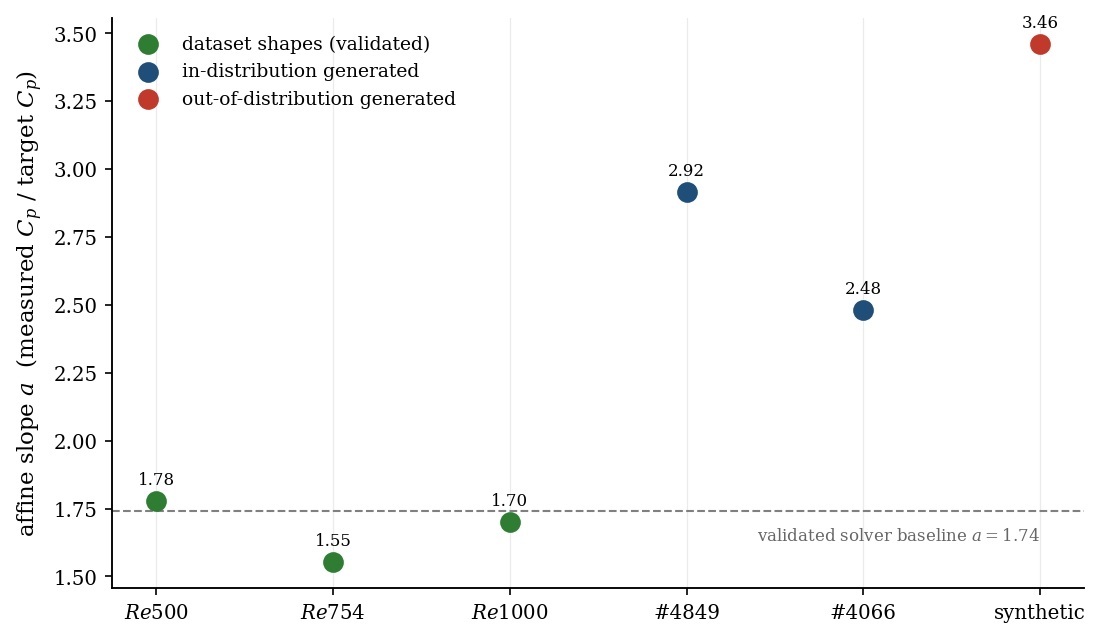
\includegraphics[width=0.8\linewidth]{EXP-042_creep_ladder.png}
  \caption{Affine slope $a$, graded by the same solver, from validated dataset shapes to generated
  shapes: real dataset ellipses sit at the validated baseline ($a \approx 1.6$--1.8, dashed), while
  generated shapes --- in-distribution (\#4849, \#4066) and out-of-distribution (synthetic) --- sit well
  above it ($a \approx 2.5$--3.5), isolating the magnitude creep to the generator.}
  \label{fig:creep-ladder}
\end{figure}

\paragraph{Posterior guidance is the wrong knob out of distribution.} The intuitive fix --- Diffusion
Posterior Sampling \cite{chung2023dps}, adding a likelihood gradient from the model's own pressure head
--- makes every metric worse, swept on a fixed OOD target at constant seed so the shapes differ only by
the guidance:

\begin{table}[t]
  \centering
  \begin{tabular}{lccc}
    \toprule
    DPS weight & $C_p$ corr & affine slope $a$ & $C_d$ \\
    \midrule
    0.0 (plain CFG) & \textbf{0.860} & 3.46 & 1.59 \\
    0.3             & 0.818          & 5.22 & 2.46 \\
    0.5             & 0.807          & 5.32 & 2.33 \\
    1.0             & 0.762          & 6.48 & 3.10 \\
    \bottomrule
  \end{tabular}
  \caption{DPS guidance sweep on a fixed out-of-distribution target: $C_p$ correlation, affine slope,
  and drag coefficient all degrade monotonically with guidance weight.}
  \label{tab:dps-sweep}
\end{table}

Correlation falls while the amplitude slope and drag rise monotonically: DPS steers toward the
self-trained pressure head, which is exactly the unreliable component out of distribution, so stronger
guidance optimises the surrogate's own error. Plain classifier-free guidance is the correct OOD
configuration; the gap is not closable by a self-graded posterior.

\begin{figure}[t]
  \centering
  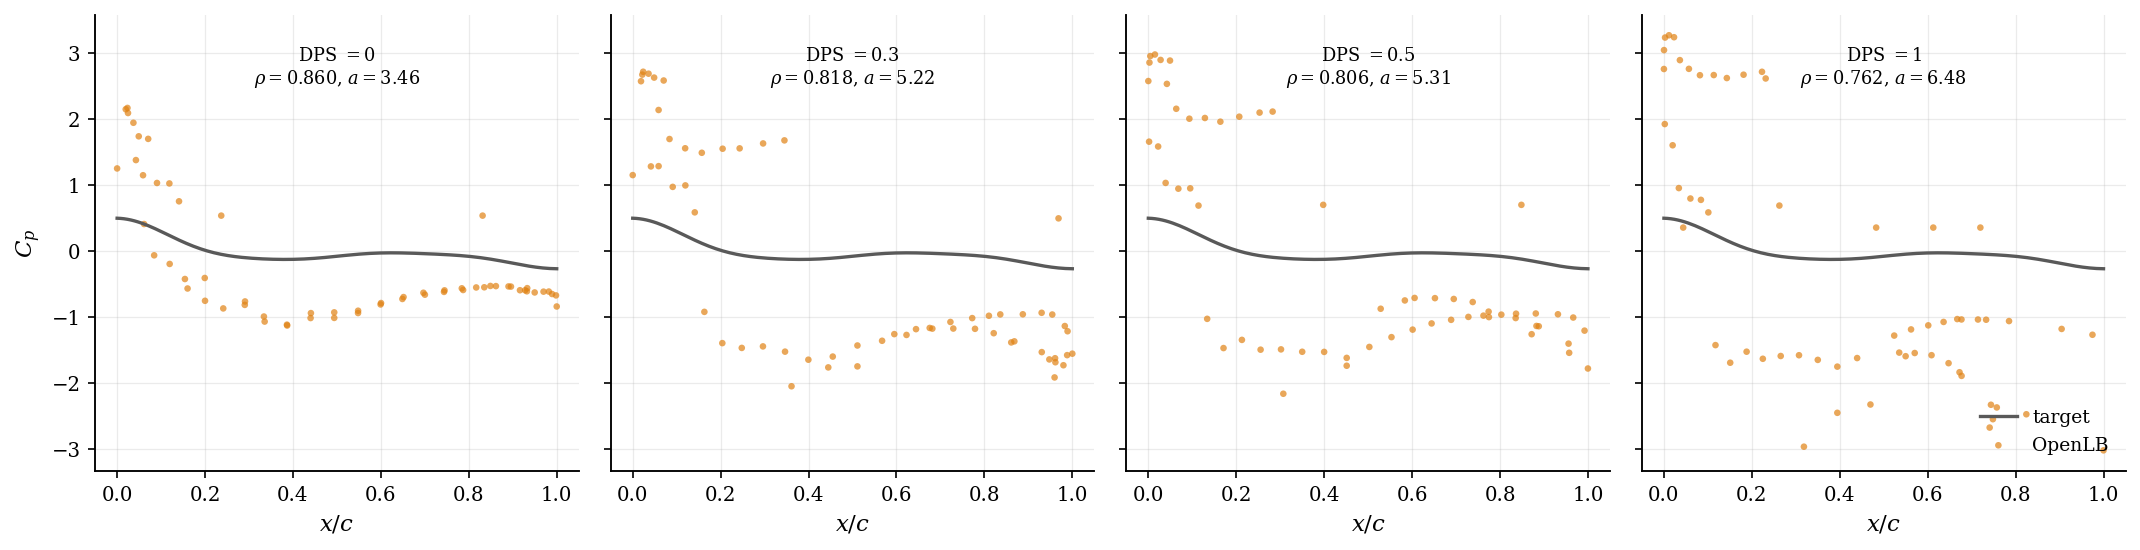
\includegraphics[width=0.8\linewidth]{EXP-041_dps_sweep.png}
  \caption{Inverse-design fidelity against DPS guidance weight: correlation falls while the amplitude
  slope and drag rise monotonically, so posterior guidance degrades true out-of-distribution fidelity.}
  \label{fig:dps-sweep}
\end{figure}

\subsection{Qualitative flow fields}

Instantaneous OpenLB fields around a generated in-distribution shape, rendered in ParaView, give
the qualitative picture behind the validation numbers. In the velocity-magnitude field the laminar
boundary layer separates off the body and rolls up into a regular von K\'{a}rm\'{a}n vortex street
--- the alternating wake that defines the Re 500--1000 shedding regime --- with accelerated flow
over the shoulders and a low-momentum wake behind the body.

\begin{figure}[t]
  \centering
  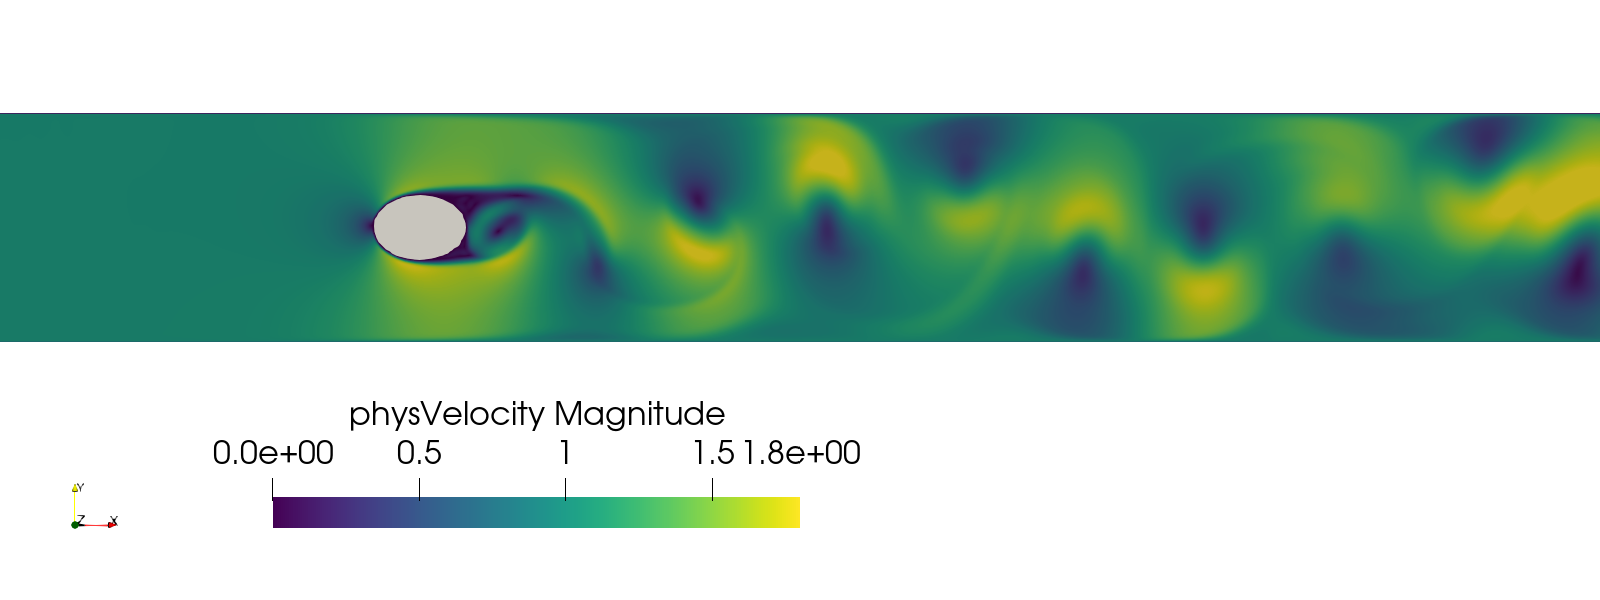
\includegraphics[width=0.8\linewidth]{report_paraview_velocity_wake.png}
  \caption{Velocity-magnitude field around a generated in-distribution shape: a laminar separation
  rolling up into a regular von K\'{a}rm\'{a}n vortex street, with accelerated shoulder flow and a
  low-momentum wake.}
  \label{fig:paraview-velocity}
\end{figure}

The pressure field at the same instant shows a high-pressure stagnation region on the upstream nose
and a train of discrete low-pressure vortex cores shed into the wake. The surface trace of exactly
this field \emph{is} the $C_p(x/c)$ curve that the inverse-design loop grades, making concrete what
the correlation numbers above are measuring.

\begin{figure}[t]
  \centering
  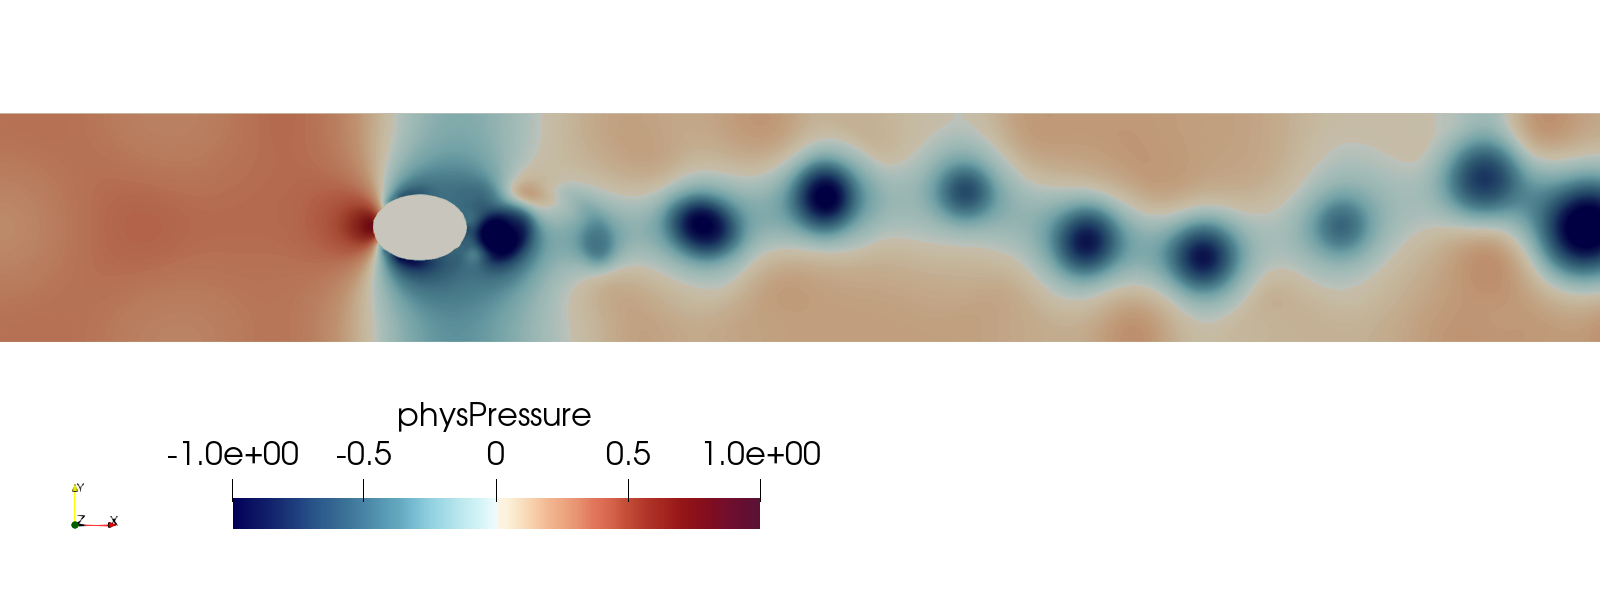
\includegraphics[width=0.8\linewidth]{report_paraview_pressure.png}
  \caption{Pressure field at the same instant: a high-pressure stagnation nose and a train of
  discrete low-pressure vortex cores in the wake, whose surface trace is the graded $C_p(x/c)$
  curve.}
  \label{fig:paraview-pressure}
\end{figure}

\section{Discussion}

\subsection{In-distribution trust versus out-of-distribution extrapolation}

The clearest message of the results is a sharp boundary between two regimes. \emph{In-distribution},
the loop is trustworthy on every axis we can test: the solver reproduces dataset pressure at
$\rho \approx 0.96$ across the whole $(Re, H)$ grid, and generated shapes hit their target morphology
at $\rho \approx 0.95$. This is a genuine, independent confirmation of inverse design --- the grading
physics shares no component with the generator, so a high correlation cannot be the model marking its
own work. \emph{Out-of-distribution}, fidelity degrades smoothly and predictably with distance from
the training manifold: morphology correlation softens from $\approx 0.96$ to $\approx 0.86$ along the
controlled $+\mathrm{PC1}$ ladder. The model interpolates within the laminar elliptical regime it has
seen and extrapolates poorly beyond it --- exactly the behaviour the independent loop was built to
expose, and a useful one to have quantified rather than assumed.

\subsection{Magnitude creep is a model-side calibration issue}

Two independent lines of evidence localise the amplitude bias to the generator, not the solver. First,
the resolution-, node-density- and roughness-controlled ladder leaves the affine slope $a$ unmoved by
any CFD or discretisation lever, with $a$ already elevated \emph{in-distribution}. Second, the
systematic OOD ladder measures $a \approx 2.0$--2.5 on generated shapes against the solver's validated
$a \approx 1.74$ on real dataset shapes run through the same pipeline --- the same solver, the same
mesh family, the same normalisation, differing only in whether the shape was generated or real. The
gap is therefore generative: the model captures pressure \emph{shape} faithfully but systematically
overshoots its \emph{amplitude}. This is why we report correlation, not absolute amplitude, as the
inverse-design verdict, and treat the slope as a calibration target to be closed model-side (for
example via the deferred physical-$Re$ conditioning) rather than a solver defect to be chased in the
CFD.

\subsection{Why posterior guidance is the wrong knob out-of-distribution}

The intuitive fix for the OOD gap --- adding a likelihood gradient from the model's own pressure head
via Diffusion Posterior Sampling \cite{chung2023dps} --- makes every metric worse, monotonically with
guidance strength. The mechanism is that DPS steers toward the \emph{self-trained} head's estimate of
the target, and out-of-distribution that head is precisely the component that is unreliable; stronger
guidance just optimises the surrogate's own error and inflates the body. This is a clean negative
result: plain classifier-free guidance is the correct OOD configuration, and the OOD gap cannot be
closed cheaply with a self-graded posterior. It must be closed by widening what the model genuinely
knows --- more diverse training data, or physically-grounded conditioning --- not by trusting the
surrogate harder.

\subsection{Limitations}

The findings above are bounded by several limitations, which also frame the next phase of work.

\paragraph{Validation framework still being verified.} All OpenLB-derived numbers are provisional
pending re-verification of the validation framework, and are flagged as such throughout. The
qualitative conclusions --- in-distribution trust, OOD decay, model-side magnitude creep, the DPS
negative --- are robust to modest shifts in the exact figures, but the precise correlations and slopes
should be read as current best estimates rather than settled values.

\paragraph{Narrow physical regime.} The entire study lives in 2D incompressible laminar flow around
elliptical cylinders at $Re$ 500--1000 (the vortex-shedding regime), with a single-family geometry
parameterised mainly by minor axis $b$. Nothing here speaks to turbulent, compressible, 3D, or
aerofoil-like flows; the demonstrated inverse-design capability is for this controlled testbed, chosen
deliberately as a tractable first target before scaling.

\paragraph{Steady-mean pressure target.} The 101 unsteady pressure timesteps per simulation are
collapsed to a single steady-mean $C_p$, discarding all temporal structure of the shedding. The model
neither conditions on nor predicts unsteady loads, so phenomena that matter aerodynamically ---
shedding frequency, fluctuating lift, phase --- are outside its scope by construction.

\paragraph{Single solver, single mesh family, no formal grid-convergence study.} Validation rests on
one lattice-Boltzmann solver with Reynolds-scaled but not formally converged resolution
($\mathrm{RES} \approx 0.2\,Re$, set for stability rather than from a grid-independence study), and
correlation is observed to taper slightly at the high-$Re$ end through genuine under-resolution. An
external benchmark (the Hron--Turek case) and a grid-convergence study remain outstanding and are
required before the solver's absolute accuracy --- as opposed to its internal consistency --- can be
claimed.

\paragraph{Conditioning is pressure-only and band-limited.} The target is encoded as just the first
$K = 8$ DCT-II modes of $C_p(x/c)$, which capture smooth low-frequency morphology but truncate sharp
pressure features; and the model conditions on $C_p$ alone, with no physical $Re$/$H$ conditioning.
Reynolds number is fixed (754) across the OOD ladder, so the present results cannot separate
$C_p$-morphology extrapolation from Reynolds extrapolation. Adding $Re$ conditioning is the deferred
next step and the natural lever on the magnitude creep.

\paragraph{OOD axis not isometric to conditioning space.} The PCA-$\sigma$ ladder only reaches genuine
OOD along $+\mathrm{PC1}$; the other principal directions stay near the training manifold regardless of
amplitude, because raw-curve PCA $\sigma$-units do not map linearly onto the DCT-conditioning space the
model sees. The controlled OOD claim is therefore strongest along $+\mathrm{PC1}$; a fully monotone,
isotropic OOD sweep requires re-parameterising the ladder directly in conditioning space.

\paragraph{Unresolved amplitude calibration.} The magnitude creep ($a$ elevated above the validated
1.74) is diagnosed but not yet fixed, so the model is an inverse designer of pressure \emph{shape}, not
of absolute pressure level. Until calibration is closed, downstream use must rely on correlation rather
than predicted magnitudes.

\paragraph{Surface roughness is cosmetic here but unquantified at scale.} Raw-versus-smoothed shapes
differ by only $\sim 0.01$ in correlation and $\sim 5\%$ in $C_d$ in the present regime, so the
characteristic boundary wobble does not corrupt the physics measured here. Whether that remains true at
higher $Re$, where thinner boundary layers are more sensitive to surface detail, is untested.

\subsection{Toward a rigorous evaluation}
\label{sec:toward-rigour}

The preliminary studies of Sections~\ref{sec:surface-quality} and earlier fixed design choices but are
not, on their own, rigorous; this section states how each would be put on a firm footing, alongside the
validation work proper.

\paragraph{Representation and connectivity.} The $k = 6$ connectivity choice rests on a single-seed
sweep on the \emph{circle} benchmark. A rigorous version would (i) repeat across several seeds and
report confidence intervals rather than point estimates, (ii) run the ablation on the \emph{aerodynamic}
dataset, where the relevant metric is the solver-graded $C_p$ correlation rather than a
radius-distribution KS distance, and (iii) sweep connectivity jointly with the layer count to rule out
confounding.

\paragraph{Surface quality.} The second-difference roughness of $r(\theta)$ is a convenient proxy, not a
standard measure. A rigorous treatment would adopt a resolution-independent curvature/spectral roughness
metric, tie it to a mesh-convergence study, and --- most importantly --- test directly whether smoothing
changes the solver-measured $C_p$/$C_d$ at the upper end of the Reynolds range, where boundary layers
are thinnest and most sensitive to surface detail. The present evidence that the wobble is cosmetic
holds only in the validated regime.

\paragraph{Out-of-distribution axis.} The PCA-$\sigma$ ladder reaches genuine OOD only along
$+\mathrm{PC1}$. A rigorous OOD protocol would define the ladder directly in the DCT-conditioning space
the model sees, so distance is monotone and isotropic in every direction, and would sample several seeds
per target to separate generative variance from systematic extrapolation error.

\paragraph{Validation framework and benchmarking.} Throughout, the OpenLB numbers are provisional
pending re-verification of the validation framework, and the solver itself has been checked only for
internal consistency (it reproduces the dataset normalisation). Establishing \emph{absolute} accuracy
requires a formal grid-convergence study and an external benchmark --- the Hron--Turek case --- which is
the immediate next validation milestone. The qualitative flow fields would likewise be promoted to
quantitative wake diagnostics (Strouhal number, separation point) compared against reference values.

\section{Conclusions}

% STUB --- draft in Year-2 paper pass

% - Phase 1 (independent physical validation) complete.
% - Phase 2: CFD-in-the-loop optimisation in the model's latent/gradient space with OpenLB as
%   ground truth.


\bibliographystyle{plainnat}
\bibliography{refs}

\end{document}
